\documentclass{FastFyp}
\begin{document}
\newcommand{\supervisor}{Mr.\ Mubasher Hussain}
\newcommand{\university}{National University of Computer and Emerging Sciences, Lahore}
\newcommand{\fyptitle}{A.R.T.E.M.I.S: Adaptive Reasoning, Task Execution and Multi-agent Intelligence System}
\newcommand{\degree}{BS}
\newcommand{\Studentone}{Hashir Rauf \hspace{1em} Roll No. 23L-2572 \hspace{1em} BS(CS)}
\newcommand{\Studenttwo}{Hira Khalid \hspace{1em} Roll No. 23L-2594 \hspace{1em} BS(CS)}
\newcommand{\Studentthree}{Syeda Doureesha Batool \hspace{1em} Roll No. 23L-2651 \hspace{1em} BS(CS)}
\date{October 6, 2026}
\renewcommand{\contentsname}{Table of Contents}

\makeatletter
    \begin{titlepage}
        
\includegraphics[width=0.2\linewidth]{Figures/nulogo.png}\hfill
        
\includegraphics[width=0.2\linewidth]{Figures/fast.png}\\
        \begin{center}
            {\large\bfseries \university}\\[7ex]
            
\includegraphics[width=0.4\linewidth]{Figures/fastlogo.png}\\[8ex]
            {\huge \bfseries  \fyptitle }\\[10ex]
            {\Studentone}\\{\Studenttwo}\\{\Studentthree}\\[4ex]
            {Supervisor: \supervisor} \\ [10ex]
            {Final Year Project}\\
            {\large \@date}
        \end{center}
    \end{titlepage}
\makeatother
\frontmatter

\newpage \thispagestyle{empty} \mbox{} \newpage

\pagestyle{empty}
\section*{\begin{center}{Anti-Plagiarism Declaration} \end{center}}
This is to declare that the above publication was produced under the:
\begin{flushleft}
\bf Title: \fyptitle
\end{flushleft}

is the sole contribution of the author(s), and no part hereof has been reproduced as it is the basis (cut and paste) that can be considered Plagiarism. All referenced parts have been used to argue the idea and cited properly. I/We will be responsible and liable for any consequence if a violation of this declaration is determined.
\\[4ex]
Date: October 6, 2026

\begin{flushright}
Name: Hashir Rauf
\\[3ex]
Signature: ..........................
\\[6ex]
Name: Hira Khalid
\\[3ex]
Signature: ..........................
\\[6ex]
Name: Syeda Doureesha Batool
\\[3ex]
Signature: ..........................

\end{flushright}

\vspace{5 cm}

\hrule

\section*{Author's Declaration}
This states Authors' declaration that the work presented in the report is their own, and has not been submitted/presented previously to any other institution or organization.
\pagebreak

\section*{Abstract}
People lose time returning to interrupted work, and the assistants capable of relieving this require broad access to a user's machine, trading away the privacy and control that make such a tool acceptable. This report presents A.R.T.E.M.I.S., a bounded, opt-in desktop assistant that operates only on folders the user has explicitly granted, deletes nothing, and routes every state-changing or outward action through preview and approval with undo available afterwards. A questionnaire of 374 respondents and 13 interviews confirmed the problem and supported the central hypothesis, with 65 percent rating a workspace-only assistant more trustworthy than a full-access one. The report specifies the requirements, architecture and design by which this restriction is enforced structurally rather than promised behaviourally.
\pagebreak

\section*{Executive Summary}
This report is the second deliverable of final year project F26-008 and documents the problem, the supporting research, the requirements and the design of A.R.T.E.M.I.S., an adaptive reasoning, task execution and multi-agent intelligence system. The project builds a desktop artificial intelligence assistant for students, developers and knowledge workers who work across many files and lose time re-establishing context after interruptions. The problem has two halves: the cost of resuming interrupted work, and the fact that the assistants capable of relieving it demand broad access to the user's machine, which many users will not accept. The central hypothesis follows from that tension, namely that restricting an assistant's scope to explicitly granted folders increases user trust and adoption without meaningfully reducing usefulness.

Foundational research tested the problem and the hypothesis before any design was committed to. A questionnaire drew 374 valid responses and 13 interviews were coded against a five-axis guide. The problem was confirmed, with 44 percent of respondents struggling to recover context after a break and 42 percent losing more than an hour a week to the surrounding friction. The hypothesis was supported, with 65 percent rating a workspace-bounded assistant more trustworthy than a full-access one, and local-first operation emerging as the most common deployment preference. Two findings shaped the design directly. Respondents divided almost evenly on whether an assistant should ask before acting, which made approval granularity a configurable setting rather than a fixed decision. They were also forgiving of a single mistake where recovery was easy, which made visible, reliable undo more important than eliminating every error.

The architecture turns the hypothesis into structure through three enforcement points. A workspace broker is the only component that resolves a path, and it canonicalises before testing containment, which is what makes traversal and symbolic link escapes impossible rather than merely discouraged. A policy engine classifies every proposed action into one of four risk tiers, where reads run automatically, reversible changes are gated by user configuration, outward actions are always gated, and destructive operations are refused because no code path to them exists. A tool dispatcher is the single point at which anything executes, and it refuses any call lacking a matching policy verdict, with every change recorded for reversal before it is made. The review also identified three limitations the project inherits rather than solves, being approval fatigue, the difficulty of detecting unfaithful generated text, and the unreliability of citations, and these are reported as known limitations throughout.

The report then proceeds from the problem and its vocabulary to the project vision, the literature and related applications, the requirements, the approach and methodology, and finally the design.
\pagebreak

\pagestyle{fancy}
\tableofcontents

\pagebreak
\listoffigures
\addcontentsline{toc}{chapter}{List of Figures}
\pagebreak
\listoftables
\addcontentsline{toc}{chapter}{List of Tables}

\mainmatter


\chapter{Introduction}
Knowledge work is rarely continuous. A student writing a thesis, a developer tracing a defect and a freelancer preparing a report all move between many files, and all of them are interrupted. When they return, the material is still on disk but the context is not: which files mattered, what had already been done, and what the next step was supposed to be must all be reconstructed by hand. The same population also carries a steady load of routine work, including organising folders, gathering material scattered across documents, and preparing correspondence, which consumes effort without advancing anything.

Artificial intelligence assistants promise to absorb this load, and to a degree they do. The difficulty is the terms on which they do it. One family of tools requires the user to direct every step, which leaves the coordination burden exactly where it was. Another family, increasingly the more capable one, asks for broad access to the user's machine, and in exchange for that access offers genuine multi-step automation. That exchange is the reason many people decline to use these tools at all. Broad access creates real exposure, and a user who cannot see what an assistant holds, cannot predict what it will do, and cannot reverse what it has done has no practical way to limit that exposure.

A.R.T.E.M.I.S., an adaptive reasoning, task execution and multi-agent intelligence system, is a desktop assistant built on the position that these two properties need not be traded against one another. The system operates only within folders a user has explicitly granted, holds nothing outside them, deletes nothing, and passes every action that changes a file or leaves the machine through a preview and approval step that the user controls. A panel called ``What ARTEMIS Knows'' reports everything the system currently holds, and every entry in it can be deleted. The project's hypothesis is that this restriction is not a sacrifice but an advantage, and that an assistant confined to a scope the user chose will be trusted, and therefore used, more readily than one that is not.

This chapter states the purpose of the document, identifies its intended audience, and defines the terms and abbreviations used throughout the report.

\section{Purpose of this Document}
The purpose of this document is to present the problem, the supporting research, the requirements and the design of A.R.T.E.M.I.S., a bounded and opt-in desktop artificial intelligence assistant that helps users manage daily work inside folders they explicitly grant to it. The document records the work completed in the first phase of the project and establishes the specification against which the implementation is built and evaluated.

The project sets out to answer one research question: can an assistant whose scope is restricted to explicitly granted workspaces deliver effective multi-step task automation while measurably improving user trust, and without meaningfully reducing usefulness? The hypothesis under test is that such a restriction increases trust and adoption at an acceptable cost to capability.

The objectives that follow from this question are to build a desktop assistant that operates strictly within granted workspaces, to reduce the time and effort users spend on resumption and routine file work, to keep the user in control of every consequential action through preview, approval and undo, and to evaluate the resulting system on task completion time, cognitive workload, usability and trust.

The methods used in this phase were a questionnaire of 374 respondents and 13 coded in-person interviews, a structured review of 26 studies across seven themes, and an architectural design derived from both. The document is bounded in two respects that should be stated plainly. It specifies and designs the system rather than reporting its evaluation, because the evaluation belongs to the second phase of the project. It also assumes a single-user desktop context throughout, so multi-user and enterprise deployment are outside its scope.

\section{Intended Audience}
This document is written primarily for the final year project evaluation panel and the project supervisor, who assess whether the problem is real, whether the research supports the proposed solution, and whether the design is sound and achievable within the remaining time. For this audience the document emphasises justification, and each significant design decision is traced to the finding that produced it.

A second audience is the project team itself. The specification and design in Chapters 4 and 6 are the reference the implementation is built against, and the requirements are written to be verifiable so that a completed feature can be checked against them rather than judged informally.

A third audience is any developer who later extends the system. For this reader the architecture chapter identifies the invariants that must survive modification, in particular that path resolution occurs in exactly one component and that execution occurs in exactly one other.

\section{Definitions, Acronyms, and Abbreviations}
The following terms are used throughout this report.

\textbf{ARTEMIS}: Adaptive Reasoning, Task Execution and Multi-agent Intelligence System, the assistant specified by this report\\
\textbf{Workspace}: a folder the user has explicitly granted, and the only region of the filesystem the system may access\\
\textbf{Grant}: the record of a user's decision to opt a folder in as a workspace, carrying its permission level and cloud policy\\
\textbf{Workspace Broker}: the single component that resolves a logical reference into a real filesystem path, or refuses\\
\textbf{Policy Engine}: the component that classifies each proposed action into a risk tier and decides whether it runs, is gated, or is refused\\
\textbf{Tool Dispatcher}: the single component permitted to execute an action\\
\textbf{Plan}: an ordered set of proposed actions produced by the planner, and the unit at which approval and undo operate\\
\textbf{Tool Call}: one proposed action within a plan\\
\textbf{Verdict}: the policy engine's decision about a single tool call\\
\textbf{Risk Tier}: the classification of an action as read, reversible, outward or destructive, written T0 to T3\\
\textbf{Egress}: the transfer of any data out of the user's machine\\
\textbf{Approval Gate}: the point at which a proposed action is held until the user approves or rejects it\\
\textbf{Undo Journal}: the record of how to reverse each change, written before that change is made\\
\textbf{Audit Log}: the append-only, hash-chained record of every proposal, refusal and action\\
\textbf{Canonicalisation}: resolving a path to its true location, following symbolic links and relative segments\\
\textbf{AI}: Artificial Intelligence\\
\textbf{LLM}: Large Language Model\\
\textbf{RAG}: Retrieval-Augmented Generation\\
\textbf{STT}: Speech to Text\\
\textbf{TTS}: Text to Speech\\
\textbf{VAD}: Voice Activity Detection\\
\textbf{CLI}: Command Line Interface\\
\textbf{GUI}: Graphical User Interface\\
\textbf{PWA}: Progressive Web Application\\
\textbf{API}: Application Programming Interface\\
\textbf{UI}: User Interface\\
\textbf{UX}: User Experience\\
\textbf{FYP}: Final Year Project\\
\textbf{MVP}: Minimum Viable Product\\
\textbf{SDG}: Sustainable Development Goal\\
\textbf{SRS}: Software Requirement Specification\\
\textbf{DO}: Durable Object, a stateful coordination primitive used in the optional remote access plane

\section{Conclusion}
This chapter has introduced the problem of interrupted knowledge work and the unacceptable trade-off that current assistants impose on users who wish to address it, and has set out the purpose, audience and vocabulary of the report. The remainder of the document proceeds as follows. Chapter 2 states the project vision, including its goals, scope, constraints, sustainable development goal alignment and stakeholders. Chapter 3 reviews the literature and related applications across seven themes and identifies where this project fills a gap and where it inherits a limitation. Chapter 4 specifies the software requirements, covering features, functional and non-functional requirements, use cases and risks. Chapter 5 describes the proposed approach and the development methodology. Chapter 6 presents the high-level and low-level design, including the architecture, the domain model and the policies that govern implementation.


\chapter{Project Vision}
This chapter states what the project is for. It describes the problem domain, states the problem and its constituent sub-problems, sets out the goals and objectives, bounds the scope, identifies the sustainable development goal the project targets, records the constraints under which it operates, notes the business opportunity, and describes the stakeholders and their characteristics. The evidence cited throughout is drawn from the project's own foundational research, a questionnaire of 374 respondents and 13 coded interviews, which is reported more fully in Chapter 3.

\section{Problem Domain Overview}
The domain is personal knowledge work carried out on a desktop computer by one person working across many files. The population consists of students, developers, freelancers and employed knowledge workers, and the defining characteristic of their work is that it is distributed across artefacts and interrupted in time. A single piece of work will typically span documents, source files, notes, messages and web material, and will be picked up and put down repeatedly over days or weeks.

Our questionnaire confirms that this describes the target population accurately. Of 374 respondents, 82 percent do multi-file project work daily or a few times a week, and none do it less often than a few times a month. Figure~\ref{fig:profile} shows the composition of the sample and the frequency of this work.

\begin{figure}[!ht]
    \centering
    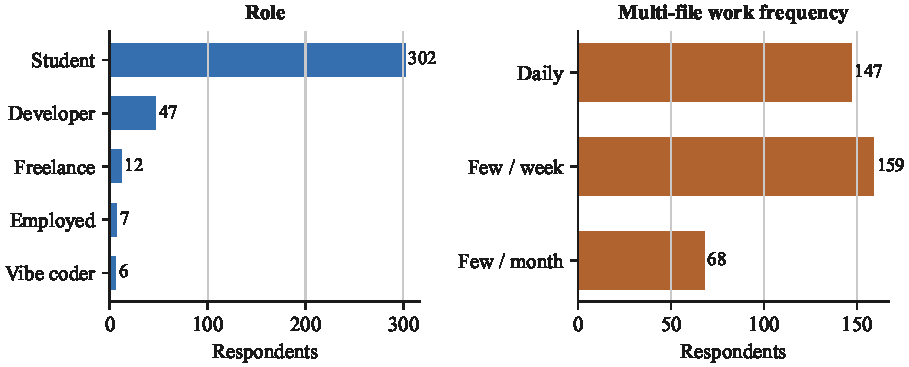
\includegraphics[width=\textwidth]{Figures/fig_profile.pdf}
    \caption{Respondent role and frequency of multi-file project work. The sample is student-heavy, which matches the intended early-adopter profile, and multi-file work is frequent across every group.}
    \label{fig:profile}
\end{figure}

Within this domain ARTEMIS is a desktop assistant that operates on folders the user has explicitly granted. It restores context after an interruption by reporting what was recently active and what was intended next. It organises files by proposing a set of moves the user previews and approves. It gathers material from several documents into a synthesis in which each claim carries a citation back to its source. It observes repeated manual sequences and offers, after the third repetition, to automate them. It reads source code to explain errors and proposes fixes as a difference the user reviews. It searches the web on demand, prepares electronic mail for approval before sending, and drafts documents as new files. Each of these is available by voice as well as by typing.

The system holds a boundary around all of this. It cannot resolve a path outside a granted workspace, it has no operation that deletes user data, and every action that changes a file or leaves the machine is held for the user's approval before it runs.

\section{Problem Statement}
Users of multi-file knowledge work lose substantial time and effort re-establishing context after interruptions and performing routine file and correspondence tasks, and the artificial intelligence assistants capable of relieving this burden require broad, unbounded access to the user's machine, which creates privacy exposure, risk of unintended modification and loss of user control that many users are unwilling to accept.

\section{Problem Elaboration}
The problem separates into five sub-problems, each of which the project addresses in a distinct way.

The first is loss of context after interruption. When a user returns to work after a break of a day or more, the information needed to resume is distributed across the filesystem, the applications that were open, and the user's own memory, and the last of these is the component that fails. Our questionnaire found that 44 percent of respondents often or always struggle to remember what they were doing when they return to a project, and only 7 percent never do. Figure~\ref{fig:return} shows this distribution.

\begin{figure}[!ht]
    \centering
    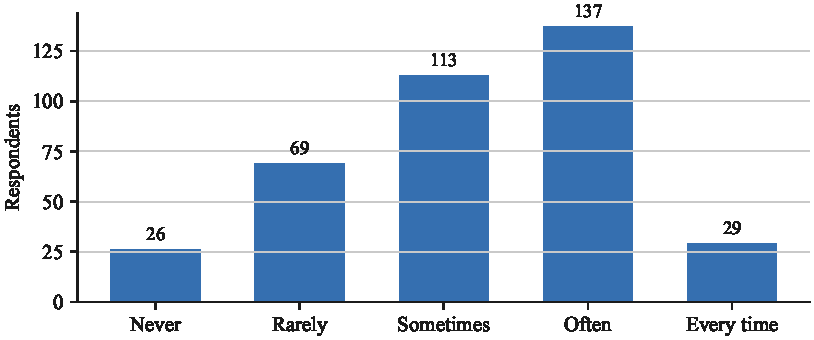
\includegraphics[width=0.82\textwidth]{Figures/fig_return_struggle.pdf}
    \caption{Frequency with which respondents return to a project after a break of a day or more and struggle to recall what they were doing or what to do next.}
    \label{fig:return}
\end{figure}

The second is accumulated file disorder. Organisation decays continuously and is repaired only occasionally, so the filesystem drifts steadily away from any structure that would make material easy to find. Among our respondents, 59 percent agreed or strongly agreed that their folders become disorganised faster than they can manually clean them, with a mean of 3.6 on a five-point scale.

The third is the cost of routine manual work, which is individually small and collectively significant. Respondents estimated the total weekly time lost to reorientation, tidying, repeated manual tasks and searching scattered notes, and 42 percent placed it above an hour a week with 14 percent above three hours. Figure~\ref{fig:time} shows the distribution, whose mode falls between thirty and sixty minutes. This is steady friction rather than crisis, which is the correct way to understand what the system is relieving.

\begin{figure}[!ht]
    \centering
    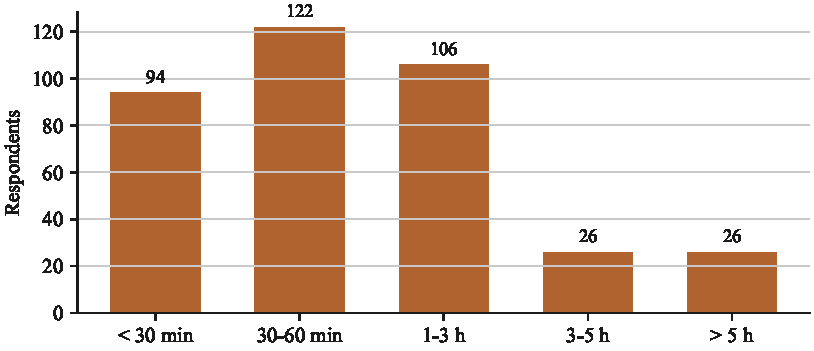
\includegraphics[width=0.82\textwidth]{Figures/fig_time_lost.pdf}
    \caption{Estimated total time lost per week to reorienting after breaks, tidying files, repeating manual tasks and searching scattered notes.}
    \label{fig:time}
\end{figure}

The fourth is that this work remains unautomated for reasons of trust and knowledge rather than absence of need. When asked why they had not already automated these tasks, 36 percent of respondents cited not trusting automation to do it correctly and 28 percent cited not knowing how, as shown in Figure~\ref{fig:whynot}. The tasks exist and are recognised; what is missing is an instrument the user is willing to point at them.

\begin{figure}[!ht]
    \centering
    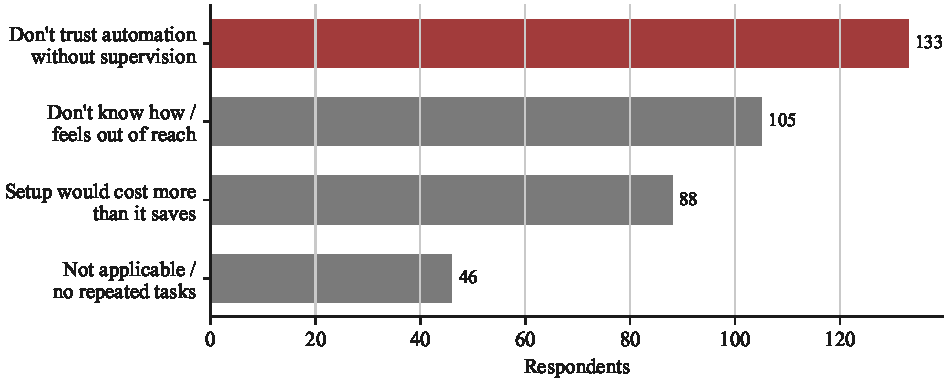
\includegraphics[width=0.82\textwidth]{Figures/fig_why_not_automated.pdf}
    \caption{Reasons respondents gave for not already automating repeated manual tasks. Distrust of automation and lack of know-how dominate.}
    \label{fig:whynot}
\end{figure}

The fifth is the access bargain that existing assistants impose, which is the sub-problem that distinguishes this project. A capable assistant is generally granted wide access to the machine, and the user is then unable to determine what it holds, what it may do, or how to reverse what it has done. Our questionnaire tested the alternative directly and found that 65 percent of respondents rate an assistant confined to explicitly added files as meaningfully more trustworthy than one with full access, with a mean of 3.8 on a five-point scale.

\section{Goals and Objectives}
The goal of the project is to demonstrate that a bounded, opt-in assistant can deliver useful multi-step automation while measurably improving user trust and preserving user control.

The objectives that realise this goal are as follows.

\begin{itemize}
    \item To develop a desktop assistant that operates strictly within folders the user has explicitly granted, such that access outside a grant is structurally impossible rather than merely prohibited
    \item To reduce the time and effort users spend resuming interrupted work and performing routine file, document and correspondence tasks
    \item To keep the user in control of every consequential action by routing it through preview, approval and undo
    \item To guarantee that the system deletes no user data, by providing no code path to a destructive operation
    \item To make everything the system holds visible and individually deletable through a disclosure panel
    \item To support voice as a complete interaction mode subject to the same approval gates as typing
    \item To evaluate the system on task completion time, cognitive workload, usability and trust, and to report inherited limitations honestly
\end{itemize}

\section{Project Scope}
The scope of this project is to design, build and evaluate a desktop assistant that helps a single user manage daily work within explicitly granted workspaces. The system will allow the user to:

\begin{itemize}
    \item Grant a folder as a workspace, and revoke it so that everything derived from it is removed
    \item Resume interrupted work by reviewing what was recently active and what was intended next
    \item Tidy a folder by previewing and approving a proposed set of moves
    \item Synthesise notes across several documents with each claim traceable to its source
    \item Receive an offer to automate a manual sequence after it has been repeated three times
    \item Ask questions about source code and receive explanations and proposed fixes as differences
    \item Search the web on demand
    \item Draft electronic mail and send it only after approving the draft
    \item Draft documents, always written as new files
    \item Perform any of the above by voice as well as by typing
    \item Inspect everything the system holds, and delete any part of it
    \item Reverse an approved plan as a single unit
\end{itemize}

The system will be implemented in Python. Multi-step plans will be produced using LangGraph~\cite{ref:langgraph}, which provides an explicit pause point before any workspace-changing or outward call. Language model access will be local-first through Ollama~\cite{ref:ollama}, with an optional and per-workspace cloud fallback. Persistence will use local SQLite~\cite{ref:sqlite} together with a per-workspace vector index. The interface will comprise a command line surface and a local graphical control panel.

The project deliverables will be:

\begin{itemize}
    \item A working desktop assistant implementing the features above
    \item This specification and design document, and the evaluation report that follows it
    \item A user manual
    \item A test suite covering the boundary, policy, approval and undo guarantees
\end{itemize}

The project scope does not include the following:

\begin{itemize}
    \item Access to any part of the filesystem outside a granted workspace
    \item Deletion or unsnapshotted overwriting of user data
    \item Autonomous action, meaning any file change or outward action taken without approval
    \item Background browsing, screen recording, keystroke capture or always-on audio recording
    \item Mobile applications, beyond the optional remote control surface described in Chapter 6
    \item Multi-user, shared or enterprise deployment
    \item Hosting user data on any project-operated server
\end{itemize}

\section{Sustainable Development Goal (SDG)}
The project targets Sustainable Development Goal 9, Industry, Innovation and Infrastructure, and in particular target 9.5, which concerns enhancing scientific research and upgrading technological capabilities~\cite{ref:sdg}. The complete list of goals is shown in Figure~\ref{fig:sdg}.

The project's contribution to this goal is its local-first design. The system's default configuration performs its work using a model running on the user's own machine, which means the capability it provides does not depend on continuous connectivity to a data centre, on a subscription, or on the user's willingness to transmit personal documents to a third party. This matters for the population the project targets. Students and independent practitioners, particularly in regions where connectivity is intermittent or costly, are precisely the users for whom a cloud-dependent assistant is least accessible, and a local-first assistant extends a current technological capability to them on terms they can meet. Our own data supports the preference: local-first operation was the single most common deployment choice among respondents at 40 percent, against 22 percent who actively preferred cloud.

The project also contributes to Goal 8, Decent Work and Economic Growth, through target 8.2 on productivity through technological upgrading, since the system's purpose is to remove recurring friction from knowledge work and return that time to substantive activity.

\begin{figure} [!h]
    \centering

\includegraphics[width=0.8\textwidth]{Figures/Picture1}
    \caption{The seventeen United Nations Sustainable Development Goals that may be targeted by a final year project, shown as a grid of seventeen numbered coloured tiles, each combining the goal number, its short title and a representative icon. This project targets Goal 9, Industry, Innovation and Infrastructure, and secondarily Goal 8, Decent Work and Economic Growth.}
    \label{fig:sdg}
\end{figure}

\section{Constraints}
The project operates under the following constraints, each of which shapes the design presented in Chapter 6.

\begin{itemize}
    \item The system must run on a typical student laptop, which bounds the size of the local language model, the resident memory footprint and the acceptable index size
    \item Core operation must not require internet connectivity, so any capability that depends on the network must degrade to a stated limitation rather than an error
    \item User data must not leave the machine except under an explicit per-workspace opt-in, which places the egress decision in the model router rather than in any feature
    \item The system must hold no inbound listening port beyond the loopback interface, so the optional remote plane must dial outward rather than accept connections
    \item Credentials must reside in the operating system keyring and never on disk in the system's own storage tree
    \item The project must be completed by a team of three within two academic semesters, which requires that the highest-risk components be built and validated early
    \item The evaluation must be conducted with participants drawn from a single institution's networks, which bounds the generalisability of its conclusions
\end{itemize}

\section{Business Opportunity}
The assistant market is presently divided between tools that are capable but demand broad access and tools that are constrained but require step-by-step direction. The opportunity this project addresses lies between them, and our data indicates that the gap is occupied by real demand rather than by a hypothetical preference: a majority of respondents rated a bounded assistant as more trustworthy, and distrust of automation was the single most common reason given for not having automated this work already.

Three conditions make the opportunity actionable. Local language models have become capable enough to run useful inference on consumer hardware, which makes local-first operation practical rather than aspirational. Regulatory and personal sensitivity to data handling continues to rise, which increases the value of an assistant that can state precisely what it holds. The target population is already familiar with assistants, since 77 percent of our respondents have used one, so the product does not have to establish the category.

The corresponding risk is differentiation, and our data identifies it plainly. A recurring theme in free-text responses was that the concept appeared already covered by existing developer assistants. The answer is the bounded workspace and local-first operation, and the finding indicates that this must be stated explicitly in the product rather than left for the user to infer.

\section{Stakeholders Description/ User Characteristics}
The users of this system are individuals performing knowledge work on their own machines, together with the roles involved in evaluating and maintaining the project.

\subsection{Stakeholders Summary}
Table~\ref{tab:stakeholders} identifies each stakeholder, their role with respect to the system, and their principal concern.

\begin{table}[!ht]
\centering
\caption{Stakeholders, their roles with respect to the system, and the primary concern each brings to it.}
\label{tab:stakeholders}
\begin{tabular}{|p{3.2cm}|p{5.0cm}|p{5.6cm}|}
\hline
\textbf{Stakeholder} & \textbf{Role} & \textbf{Primary concern} \\
\hline
Student & Primary user. Works across documents, notes and source files on a personal laptop, frequently interrupted. Represents 81 percent of the research sample. & Recovering context quickly; keeping personal and academic files private; no configuration burden. \\
\hline
Developer & Primary user. Works across source files and documentation, and is the principal user of the code assistant. Represents 13 percent of the sample. & Correctness of proposed changes; never having code modified without review. \\
\hline
Freelancer or knowledge worker & Primary user. Manages client documents and correspondence. & Confidentiality of client material; reliable correspondence drafting with approval. \\
\hline
Project supervisor & Assesses the project's academic soundness and progress. & Traceability of design decisions to evidence; feasibility within the timeline. \\
\hline
Evaluation panel & Assesses the delivered project against its stated objectives. & Whether the hypothesis was tested and whether limitations are stated honestly. \\
\hline
Development team & Designs, implements and evaluates the system. & Preserving the architectural invariants under change; completing the scope in time. \\
\hline
Future maintainer & Extends the system after the project concludes. & Locating the enforcement points; understanding which properties must not be broken. \\
\hline
\end{tabular}
\end{table}

\subsection{Key High-Level Goals and Problems of Stakeholders}
The primary users share a single high-level goal, which is to spend less time on the mechanics of their work and more on its substance, and they share a single high-level problem, which is that the tools capable of granting this require a degree of access they are not prepared to give. Our research refines this general statement in four respects that bear directly on the design.

Users are divided on how much they wish to be asked. The questionnaire presented a choice between an assistant that seeks approval before every file change or outward action and one that acts on reasonable requests and permits review and undo afterwards. The split was 192 to 182, shown in Figure~\ref{fig:pref}. No single interaction model satisfies this population, and approval granularity is therefore specified as a user-configurable setting in Chapter 4 rather than fixed in the design.

\begin{figure}[!ht]
    \centering
    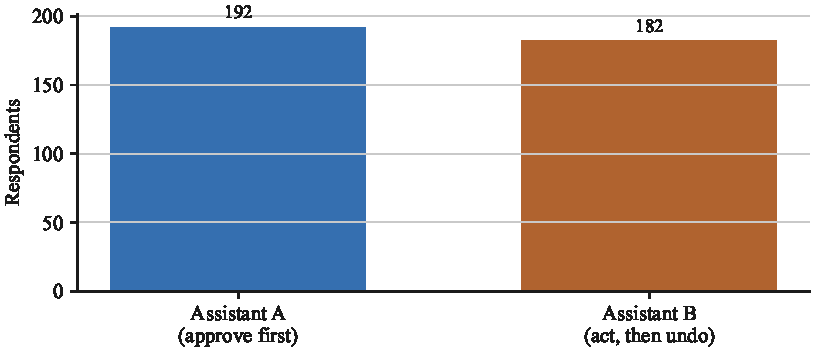
\includegraphics[width=0.72\textwidth]{Figures/fig_assistant_pref.pdf}
    \caption{Preference between an assistant that asks for approval before every file change or outward action and one that acts automatically with review and undo afterwards. The population is close to evenly divided.}
    \label{fig:pref}
\end{figure}

Users will tolerate a mistake if they can reverse it. Asked what a single wrong or unwanted suggestion would do to their usage, 65 percent said they would continue using the system, some with increased caution, and only 10 percent would abandon it. This finding establishes that a visible and reliable undo is more valuable than an unattainable perfection, and it is why the undo journal is specified as a critical component rather than a convenience.

Users will stop for reasons of fit rather than friction. The most frequently predicted reasons for abandoning the system after a week were that it did not fit existing habits, at 27 percent, and that it made a mistake the user could not trust it to avoid again, at 24 percent. Approval fatigue was the smallest named risk at 10 percent. This tempers a natural design instinct: reducing the number of prompts addresses the least common concern and would erode the trust that the approval model provides.

Users want the system to learn their structure, which is a request the bounded design must accommodate carefully. The most frequently requested capability not already planned was that the assistant learn the user's folder organisation over time. This is specified as per-workspace memory, visible and deletable in the disclosure panel, so that personalisation remains inside the bounded-scope guarantee rather than quietly widening it.


\chapter{Literature Review / Related Work}
This chapter reviews the research literature and the existing applications relevant to the project. The review covers 26 studies organised into seven themes, each corresponding to a capability or a guarantee the system must provide. For each theme the chapter summarises the work, analyses its strengths and weaknesses, and states the relationship to the proposed system. The chapter closes by identifying where the project genuinely fills a gap, where it fills one partially, and where it inherits a limitation it cannot claim to have solved.

\section{Definitions, Acronyms, and Abbreviations}
The following terms are used specifically within this chapter, in addition to those defined in Chapter 1.

\textbf{Agentic system}: a system in which a language model plans a sequence of steps and invokes tools to carry them out, rather than only producing text\\
\textbf{Human-in-the-loop}: an arrangement in which a person approves or corrects a system's proposed action before it takes effect\\
\textbf{Prompt injection}: an attack in which instructions embedded in retrieved content are treated by a model as commands from the user\\
\textbf{Hallucination}: generated content that is not supported by the source material it purports to summarise\\
\textbf{Attribution}: the property that a generated statement is genuinely supported by the source it cites\\
\textbf{Faithfulness}: the consistency of a generated summary with the document it summarises\\
\textbf{Approval fatigue}: the decline in scrutiny that occurs when a user is asked to approve actions frequently\\
\textbf{Privilege separation}: an architectural defence that isolates a trusted component from untrusted data or code

\section{Detailed Literature Review}
The review is organised into seven themes. Themes one through three concern the system's core behaviour, covering task resumption, bounded agents and trust, and agentic planning. Themes four and five concern two specific capabilities, voice interaction and code assistance. Themes six and seven concern the correctness of generated text, covering hallucination and citation accuracy.

\subsection{Task Interruption and Resumption}
Work on this problem begins with an observational finding. A field study of ordinary office computer use established that when people are pulled away from a task, visible on-screen cues such as a window left open rather than minimised are what enable them to resume it later~\cite{ref:iqbal2007}. The study was conducted in real working conditions rather than in a laboratory, and it stopped at diagnosis: no system was proposed for the case where leaving a window open ceases to be practical, such as after a restart or a gap of several days.

Later work converted this diagnosis into a tool. ScreenTrack records a background time-lapse of the screen and allows a user to scroll through it visually to locate and reopen something they remember seeing, on the reasoning that people recall sequences of visual scenes more readily than file names or timestamps~\cite{ref:hu2020}. In a controlled laboratory study it performed well for recent and visually distinct activity.

The strengths and weaknesses of this pair are complementary. The field study's strength is ecological validity, and its weakness is that it produced no intervention. ScreenTrack's strength is that it operationalises the finding, and its weaknesses were acknowledged candidly by its authors: retrieval slows as the history lengthens, the approach depends on tasks being visually distinguishable and so suits text-heavy work poorly, and it was never tested in prolonged multi-application use. There is also an evident tension between a continuous screen recording and the privacy expectations of the users this project targets.

The relationship to the proposed work is one of deliberate divergence rather than extension. The resumption feature specified in this report does not record the screen at all. It operates from the file index and from notes the user has written, matching on file name, recency and explicit text, which makes it independent of whether two screens resemble one another. Because a workspace is bounded by construction, the feature also avoids the problem of searching a long history, since only a short list of recent and relevant items exists to present. The honest qualification is that the resumption benefit remains a design claim rather than a demonstrated one, since the system has not undergone field validation comparable to the original study.

\subsection{Bounded Artificial Intelligence Agents and Trust}
A separate line of work asks how an agent's autonomy can be confined within limits a person can trust. One direction is developer-facing. A trace-based assurance framework logs every action an agent takes as a structured trace with machine-checkable contracts attached to each step, so that a violation can be traced to an exact point and replayed deterministically, mediating each action as allow, rewrite or block according to per-agent capability limits~\cite{ref:paduraru2026}.

A recent security survey examines the same space from the perspective of systems that depend on human sign-off~\cite{ref:kim2026}. It analyses privilege separation as an architectural defence, drawing an analogy to the separation an operating system maintains between a trusted kernel and untrusted programs, and applies this to isolating a planning component from untrusted external data. It then examines the limits of human-in-the-loop approval itself, and its conclusion is unfavourable: frequent approval prompts produce decision fatigue that undermines the safety benefit they exist to provide, and most users lack the background to judge what they are being asked to approve, so they either approve risky actions without real scrutiny or reject harmless ones. The survey names this as an open problem and offers no solution.

The strength of this body of work is that the machinery for bounding an agent already exists and is well understood. Its weakness, for present purposes, is that it is built for organisations with security staff and supporting infrastructure rather than for one person running an assistant on their own machine. The assurance framework is also notable for having no mechanism to undo an action once it has run.

The relationship to the proposed work runs in both directions. This project's workspace model is a plain-language rendering of the same principles: a folder the user selects rather than a sandbox an administrator defines, and a readable preview rather than a machine-checked contract. Against the assurance framework the project adds precisely what that framework lacks, which is reversal after the fact, and this is among the most direct correspondences in the review. Against the security survey the project must concede a point rather than claim one. It does not solve approval fatigue. It relies on the same mechanism the survey identifies as unresolved, and nothing in the current design distinguishes a routine approval from a risky one or reduces prompts as trust accumulates. This limitation is inherited by choosing this approach at all, and the evaluation must test for it directly rather than assume the bounded workspace dissolves it.

\subsection{Agentic Reasoning, Planning and Undo}
A substantial body of work has moved language models beyond producing text toward reasoning about a goal, planning steps and acting on them. Reflexion allows an agent to evaluate its own past attempts, write verbal reflections and store them as episodic memory to improve later attempts without retraining, improving performance on decision-making, reasoning and coding tasks~\cite{ref:shinn2023}. Toolformer takes a narrower approach, teaching a model in a largely self-supervised manner when and how to call an external tool such as a calculator or a search engine~\cite{ref:schick2023}. Generative Agents extends the memory-and-reflection idea further, demonstrating that a population of agents can behave coherently over simulated days by storing, retrieving and reflecting on experience, while also reporting failures including incorrect retrieval and fabricated memory detail~\cite{ref:park2023}. ReAct interleaves reasoning, acting and observing within a single loop and shows that the combination improves both performance and interpretability, while proving prone to repetitive action loops and poor recovery when an action returns an unhelpful result~\cite{ref:yao2023react}. Tree of Thoughts permits a model to search across multiple reasoning paths and backtrack from unpromising ones, producing substantial gains on puzzle-style tasks at a real computational cost~\cite{ref:yao2023tot}.

The strength of this literature is that it establishes reasoning, tool use and reflective memory as a workable substrate for agent behaviour. Its shared limitation is the setting in which each system is evaluated: Reflexion on its own past attempts, Toolformer on isolated tool calls it cannot readily chain, Generative Agents within a sandbox world, and ReAct and Tree of Thoughts on benchmark tasks. None maintains a bounded workspace for a real user across ordinary interrupted work, and none requires the kind of approval that would render consequential actions reversible.

The proposed work is positioned in that gap. It adopts the underlying combination of reasoning, tool use and memory but directs it at a user's actual files, notes and stated intentions rather than at the agent's own history or a simulated environment, and it wraps the resulting multi-step plans in preview, approval and undo, which none of these systems provide. The failure modes this literature reports are also a direct warning. Fabricated memory and repetitive reasoning loops describe precisely the errors the resumption and synthesis features must guard against, and they argue for keeping the number of unsupervised steps between user checkpoints small rather than assuming that a longer autonomous chain is safe.

\subsection{Voice Interaction Parity}
This theme concerns whether people can carry out practical computer work by voice as effectively as by typing, and how voice interaction should be evaluated. Two systematic reviews establish the state of the field. The first conducts a bibliometric analysis of user experience with voice interfaces and proposes a classification of six research categories, identifying voice-related factors including gender, accent, personality and style~\cite{ref:deshmukh2024}. The second reviews voice assistant usability against the ISO 9241-11 framework of effectiveness, efficiency and satisfaction~\cite{ref:dutsinma2022}.

Three empirical studies supply concrete design guidance. One demonstrates that speech carries a real-time signal of user experience that post-hoc questionnaires do not capture, with features such as pause duration and disfluency rate serving as supplementary measures~\cite{ref:ma2026}. Another examines spoken indicators during waiting periods, finding that a long wait is best handled by an indicator that both explains what is happening and introduces light humour, whereas for a short wait either alone suffices and additional information increases load~\cite{ref:zhang2025}. A third addresses response delay in free-form conversation with virtual agents, finding natural conversational fillers preferable to artificial tones~\cite{ref:wang2025}.

The strength of this literature is that it supplies usable thresholds and design rules, including a four-second latency target. Its weakness, which both reviews state, is that voice usability is studied in fragments and that standard usability metrics omit voice-specific concerns such as trust and cognitive load.

The relationship to the proposed work is twofold. For design, the waiting-indicator and filler findings govern how the voice mode behaves while a plan is being produced, which must be a spoken explanatory indicator rather than silence or a generic tone. For evaluation, the literature's agreement that voice as a complete interaction mode over practical multi-step tasks is under-explored establishes the contribution: this project compares voice against typing on ease of use, task time, cognitive workload and trust. The speech-analysis technique is an optional enhancement to that evaluation rather than a design requirement.

\subsection{Code Assistance with Human Review}
Five studies address the conditions under which language model assistance with code is useful. HULA demonstrates a plan, generate and human-approve loop in a real deployment, reporting an 82 percent plan approval rate and finding that output quality depends heavily on the quality of the input context~\cite{ref:takerngsaksiri2025}. HiLDe operates at a finer granularity, steering generation token by token, and reports two cautions: regeneration can silently overwrite earlier user edits, and presenting too many alternatives overwhelms users~\cite{ref:gonzalez2025}. A study of suggestion timing examines when an inline assistant should display a suggestion and warns against optimising for acceptance rate at the expense of usefulness~\cite{ref:mozannar2024}. A taxonomy of expert steering strategies identifies the moves by which a person redirects a model, including pointing out a specific error, clarifying a requirement and re-orienting the approach, while noting that some strategies presuppose expert knowledge~\cite{ref:chidambaram2024}. Finally, an evaluation of language models as code reviewers finds systematic overcorrection, with models inventing requirements and flagging correct code as wrong, and finds that requesting longer explanations worsens rather than improves this~\cite{ref:jin2026}.

The strength of this literature is that it validates the human-approval loop as an effective interaction model rather than a fallback. Its collective weakness, which the overcorrection study states most sharply, is that model judgement about code is useful but not trustworthy on its own, and that explanations do not make it more reliable.

The relationship to the proposed work is direct. The code assistant specified in this report adopts HULA's shape but narrows it: it reads workspace source, answers questions, explains errors and proposes a fix as a difference for the user to approve, and it neither opens pull requests nor acts across a repository. HiLDe's cautions translate into two design rules, which are to present one proposed change at a time and never to modify code the user has not approved. Because the assistant is invoked deliberately rather than offering continuous inline suggestions, the suggestion-timing problem does not arise, which is a deliberate advantage of the on-demand model. The overcorrection finding is the direct justification for never applying a change automatically, and the mitigation is the difference-plus-approval design, which reduces rather than removes the underlying limitation.

\subsection{Hallucination in Artificial Intelligence Summarisation}
Four studies trace this problem from diagnosis to meta-evaluation. The first established that hallucinated content appeared in every abstractive summarisation system tested, and identified entailment between source and output as the appropriate check~\cite{ref:maynez2020}. FactCC followed with a lightweight, trainable consistency checker, which remains the closest thing in the literature to a component that could be adopted directly~\cite{ref:kryscinski2020}. FRANK then benchmarked the available factuality metrics and found that no single metric detects every category of error~\cite{ref:pagnoni2021}. SummEdits extended the question to frontier models and found that even the strongest models judge faithfulness poorly~\cite{ref:laban2023}.

The strength of this literature is the consistency of its conclusion across a decade: hallucination is common, conventional overlap metrics do not detect it, no single detector is uniformly reliable, and models are weak judges of their own faithfulness. Its weakness from an engineering standpoint is that it supplies no complete solution, only partial detectors and the recommendation to combine them.

The relationship to the proposed work must be stated as a gap rather than a resolution. The synthesis feature operates over a small, user-selected set of documents, which is a narrower and more controlled task than open-domain summarisation and therefore presents a smaller surface for hallucination. It does not eliminate it. The current design contains no faithfulness check, so this is an open gap rather than something the bounded workspace resolves. The indicated direction is an entailment-style or FactCC-style check applied after generation, combined with retaining the user in the loop, and the SummEdits finding rules out the tempting shortcut of asking the model to check its own citations.

\subsection{Retrieval-Augmented Generation Citation Accuracy}
Three studies address whether generated text genuinely supports the sources it cites. The first supplies a usable definition of attribution, framed as whether a statement passes the test that according to the cited source, the statement is true~\cite{ref:rashkin2023}. ALCE then benchmarked the ability of models to generate text with citations and found incomplete citation to be common~\cite{ref:gao2023}. An audit of deployed generative search engines found that roughly a quarter of citations did not hold up and about half of sentences were not fully supported~\cite{ref:liu2023}.

The strength of this literature is that it supplies both a standard and empirical evidence of how far real systems fall short of it. Its weakness is that it provides a measurement apparatus rather than an enforcement mechanism.

The relationship to the proposed work is partial. The synthesis feature removes the retrieval half of the problem by having the user pre-select the documents, and the citation map described in Chapter 6 carries each chunk back to its file and line. What the current design does not do is verify that a citation supports the claim attached to it, or that every claim carries one. The audit of deployed products is the appropriate calibration here: mature products with dedicated citation engineering still fail these checks at meaningful rates, which is a reason to treat citation verification as necessary work rather than to assume that citing from a small known set is inherently safe.

\subsection{Related Development Projects and Applications}
Beyond the research literature, three families of existing application bear on the project. Inline coding assistants integrated into development environments provide continuous suggestion within a single editor, and their strength is immediacy while their limitation is that they address code alone and operate with access to whatever the editor can reach. Agentic command-line assistants execute multi-step plans across a developer's machine, and their strength is genuine multi-step capability while their limitation is the breadth of access they require and the difficulty of reversing what they have done. General-purpose conversational assistants are broadly capable but hold no persistent, structured relationship to the user's filesystem, so they cannot resume work or act on files without material being supplied to them each time.

Our own research indicates that this landscape is not merely a matter of technical comparison but of positioning. A recurring theme in free-text responses was that the proposed system appeared already covered by existing developer assistants, which establishes that differentiation must be argued explicitly. The differentiating properties are the enforced workspace boundary, local-first operation by default, the structural unavailability of destructive operations, and the disclosure panel that makes the trust claim falsifiable rather than merely persuasive.

\section{Literature Review Summary Table}
Table~\ref{tab:lr} summarises the reviewed studies, identifying the theme each addresses, the contribution it makes, its relevance to this project and its limitations.

\begin{table}[!ht]
\centering
\caption{Summary of the reviewed literature, giving the theme, contribution, relevance to this project and stated limitations of each study.}
\label{tab:lr}
{\small
\begin{tabular}{|p{2.6cm}|p{2.0cm}|p{3.6cm}|p{4.6cm}|}
\hline
    \textbf{Study} & \textbf{Theme} & \textbf{Relevance to this project} & \textbf{Limitations} \\
\hline
Iqbal and Horvitz \cite{ref:iqbal2007} & Resumption & Establishes that resumption depends on persistent cues, motivating the session resume feature & Diagnosis only; proposes no system; cues fail after restart or a multi-day gap \\
\hline
Hu and Lee \cite{ref:hu2020} & Resumption & Demonstrates a resumption tool, whose weaknesses this project avoids structurally & Slow retrieval over long histories; requires visually distinct tasks; privacy cost of screen recording \\
\hline
Paduraru et al. \cite{ref:paduraru2026} & Bounded agents & Contract mediation and capability limits inform the policy engine & Built for organisations with security staff; no mechanism to undo an executed action \\
\hline
Kim et al. \cite{ref:kim2026} & Bounded agents & Privilege separation informs the planner and dispatcher split; documents approval fatigue & Names approval fatigue as an open problem without offering a solution \\
\hline
Shinn et al. \cite{ref:shinn2023} & Agentic planning & Episodic written memory as a substrate for agent behaviour & Evaluated on the agent's own past attempts, not on real user work \\
\hline
Schick et al. \cite{ref:schick2023} & Agentic planning & Self-supervised tool invocation informs the tool contract & Isolated tool calls that cannot readily be chained into plans \\
\hline
Park et al. \cite{ref:park2023} & Agentic planning & Memory, retrieval and reflection architecture informs the memory design & Sandbox world; reports fabricated memory and incorrect retrieval \\
\hline
Yao et al. \cite{ref:yao2023react} & Agentic planning & Interleaved reasoning and acting informs the bounded reflection loop & Repetitive action loops; poor recovery from unhelpful observations \\
\hline
Yao et al. \cite{ref:yao2023tot} & Agentic planning & Search over reasoning paths informs the cycle cap on planning & Substantial computational cost; benchmark tasks only \\
\hline
Deshmukh and Chalmeta \cite{ref:deshmukh2024} & Voice & Classification of voice user experience research informs evaluation measures & Voice usability studied in fragments; no unified framework \\
\hline
Dutsinma et al. \cite{ref:dutsinma2022} & Voice & ISO 9241-11 framing of usability informs the evaluation instrument & Standard metrics omit trust and cognitive load \\
\hline
Ma et al. \cite{ref:ma2026} & Voice & Speech as a real-time experience signal; optional evaluation enhancement & Requires turn-by-turn audio capture, which this project does not plan \\
\hline
Zhang et al. \cite{ref:zhang2025} & Voice & Waiting-indicator design for periods while a plan is produced & Findings specific to the wait durations tested \\
\hline
Wang et al. \cite{ref:wang2025} & Voice & Natural fillers preferred over tones during response delay & Studied in free-form conversation rather than task execution \\
\hline
Takerngsaksiri et al. \cite{ref:takerngsaksiri2025} & Code assistance & Validates the plan, generate and approve loop at 82 percent plan approval & Output quality heavily dependent on supplied context \\
\hline
Anaya Gonzalez et al. \cite{ref:gonzalez2025} & Code assistance & Cautions against silent overwriting and excessive alternatives & Token-level granularity finer than this project requires \\
\hline
Mozannar et al. \cite{ref:mozannar2024} & Code assistance & Establishes that on-demand invocation avoids the suggestion-timing problem & Applies to inline assistants; acceptance rate is a misleading objective \\
\hline
Chidambaram et al. \cite{ref:chidambaram2024} & Code assistance & Steering taxonomy informs follow-up prompts when a fix is rejected & Some strategies presuppose expert knowledge \\
\hline
Jin and Chen \cite{ref:jin2026} & Code assistance & Direct justification for never applying a code change automatically & Models overcorrect; longer explanations worsen reliability \\
\hline
Maynez et al. \cite{ref:maynez2020} & Hallucination & Entailment identified as the appropriate faithfulness check & Hallucination present in every system tested; no complete remedy \\
\hline
Kryscinski et al. \cite{ref:kryscinski2020} & Hallucination & FactCC is the most directly adoptable consistency checker & Not currently used by this project; a stated open gap \\
\hline
Pagnoni et al. \cite{ref:pagnoni2021} & Hallucination & Warns against relying on a single faithfulness metric & No single metric detects every error category \\
\hline
Laban et al. \cite{ref:laban2023} & Hallucination & Rules out self-checking of citations by the model & Even frontier models judge faithfulness poorly \\
\hline
Rashkin et al. \cite{ref:rashkin2023} & Citation & Supplies the attribution standard for synthesis output & A standard rather than an enforcement mechanism \\
\hline
Gao et al. \cite{ref:gao2023} & Citation & Benchmarks citation generation; motivates completeness checks & Incomplete citation common even in purpose-built systems \\
\hline
Liu et al. \cite{ref:liu2023} & Citation & Calibrates expectations against deployed products & A quarter of citations unsupported; half of sentences not fully supported \\
\hline
\end{tabular}}
\end{table}

\section{Conclusion}
The reviewed literature establishes three conclusions for this project.

The project fills a genuine gap in four respects. It applies multi-step agentic planning to a bounded, user-chosen desktop workspace rather than to a simulated world, a single task or an open repository, a combination the planning literature leaves open. It makes agent memory visible and user-editable through the disclosure panel, where the reviewed systems run memory as an opaque background process and report fabricated and mis-retrieved entries. It provides reversal after a previewed action, which the assurance framework lacks entirely. It evaluates voice as a complete interaction mode over practical multi-step tasks, which both voice reviews identify as under-explored.

The project fills three further gaps partially. Its bounded capability scoping is a plain-language rendering of the capability limits and privilege separation the security literature describes, trading rigour for usability. Its resumption feature operationalises a well-established finding without having reproduced that study's field validation. Its code assistance adopts a validated human-approval loop while remaining subject to the underlying model's errors, which approval mitigates rather than removes.

The project inherits three limitations it does not solve, and these are stated here rather than deferred. It does not solve approval fatigue, which the security survey documents as an open problem in exactly the mechanism this design depends upon, and the evaluation must test for it over repeated sessions. It has no faithfulness check for synthesised text, so the narrower task reduces but does not eliminate the exposure the summarisation literature documents. It does not verify that citations support their claims or that every claim carries one, which the citation literature shows to be unreliable even in polished deployed products.

These conclusions shape the requirements in Chapter 4 and the design in Chapter 6, and they set the terms on which the evaluation in the second phase of the project must report its results.


\chapter{Software Requirement Specifications}
This chapter specifies the requirements for the system. It lists the features, states the functional requirements with their users, identifies the quality attributes and non-functional requirements, records the assumptions on which the specification rests, presents the principal use cases, states the hardware and software requirements, describes the interface and the database design, and analyses the risks. Each requirement is written to be verifiable, so that a completed implementation can be checked against it rather than assessed informally.

Requirements are identified by a prefix and number. Functional requirements are numbered FR-1 onwards, non-functional requirements NFR-1 onwards, and quality attributes QA-1 onwards.

\section{List of Features}
The system provides the following features, listed in the order in which they are built. The order is derived from measured demand, reported in Chapter 3, together with technical risk, so that the components on which every other feature depends are constructed and validated first.

\begin{itemize}
    \item Workspace management, by which a user grants a folder, inspects what the system holds about it, and revokes it together with everything derived from it
    \item Action gating, by which every proposed action is classified by risk, previewed, approved or rejected, and reversed if required
    \item Session resume, which restores the user's context after an interruption by reporting what was recently active and what was intended next
    \item Folder tidy, which proposes a set of file moves that the user previews and approves as one unit
    \item Repeated task detection, which offers to automate a manual sequence after it has been observed three times
    \item Notes synthesis, which gathers material across several documents with each claim carrying a citation to its source
    \item Code assistance, which explains errors and proposes fixes as differences for review
    \item Web search, performed only on the user's explicit request
    \item Mail composition, in which a draft is prepared and sent only after the user approves it
    \item Document drafting, which produces a first draft as a new file
    \item Speech input and output, providing voice as an alternative interaction mode subject to identical approval gates
    \item The disclosure panel, which reports everything the system currently holds and permits deletion of any part of it
\end{itemize}

The measured demand that determines this order is shown in Figure~\ref{fig:features}. Session resume, notes synthesis and folder tidy are the three most requested features, and speech is last by a wide margin, which is why it is built last.

\begin{figure}[!ht]
    \centering
    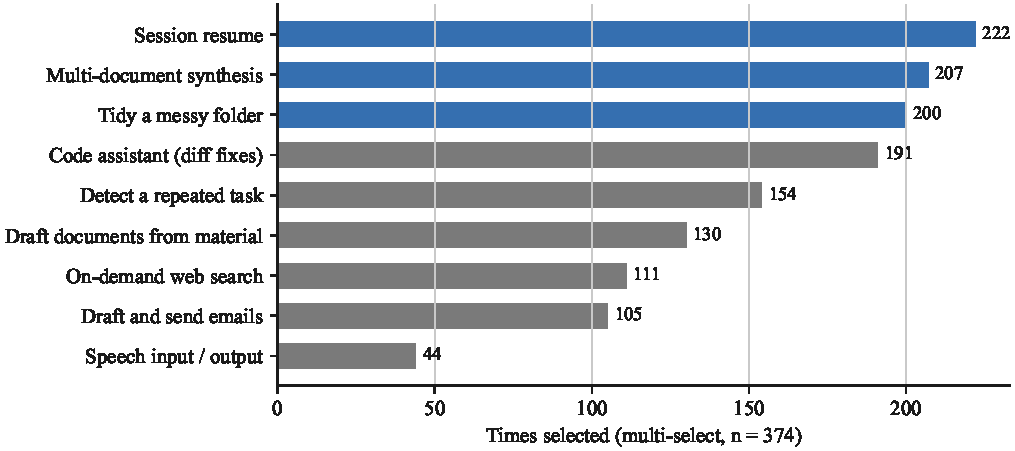
\includegraphics[width=\textwidth]{Figures/fig_features.pdf}
    \caption{Number of times each feature was selected in a forced top-three choice by 374 respondents. Demand is concentrated on session resume, notes synthesis and folder tidy.}
    \label{fig:features}
\end{figure}

\section{Functional Requirements}
The functional requirements describe the external behaviour of the system. Each is stated with the user who exercises it.

\subsection{Workspace Management}
\begin{itemize}
    \item \textbf{FR-1} The system shall allow the user to grant a folder as a workspace, recording its name, canonical root path, permission level and cloud policy. \emph{User: all primary users.}
    \item \textbf{FR-2} The system shall refuse to resolve any path whose canonical form lies outside the root of an active grant. \emph{User: all primary users, exercised indirectly.}
    \item \textbf{FR-3} The system shall canonicalise a path, resolving symbolic links and relative segments, before testing whether it is contained within a grant. \emph{User: all primary users, exercised indirectly.}
    \item \textbf{FR-4} The system shall refuse to resolve paths matching a deny list of credential and system locations, even where such a path lies within a granted folder. \emph{User: all primary users, exercised indirectly.}
    \item \textbf{FR-5} The system shall allow the user to revoke a workspace, deleting its index entries, embeddings, sessions, memory and rules, while leaving the user's own files untouched. \emph{User: all primary users.}
    \item \textbf{FR-6} The system shall maintain an index of the files within each granted workspace, updating it incrementally as files change. \emph{User: all primary users, exercised indirectly.}
\end{itemize}

\subsection{Action Gating and Recovery}
\begin{itemize}
    \item \textbf{FR-7} The system shall classify every proposed action into exactly one of four risk tiers, being read, reversible, outward and destructive. \emph{User: all primary users, exercised indirectly.}
    \item \textbf{FR-8} The system shall execute read actions within a granted workspace without requiring approval. \emph{User: all primary users.}
    \item \textbf{FR-9} The system shall hold every reversible action for approval, unless the user has previously chosen to permit that operation in that workspace without asking. \emph{User: all primary users.}
    \item \textbf{FR-10} The system shall hold every outward action for approval in all circumstances, and shall not permit this requirement to be configured away. \emph{User: all primary users.}
    \item \textbf{FR-11} The system shall refuse every destructive action, providing no approval path by which it may proceed. \emph{User: all primary users.}
    \item \textbf{FR-12} The system shall present, before any gated action, a preview stating the workspace affected, the operations proposed, the risk tier, whether anything leaves the machine, and whether anything is deleted. \emph{User: all primary users.}
    \item \textbf{FR-13} The system shall allow the user to approve, approve and remember, edit or reject a pending plan. \emph{User: all primary users.}
    \item \textbf{FR-14} The system shall scope a remembered approval to one operation within one workspace, and shall never remember an outward or destructive operation. \emph{User: all primary users.}
    \item \textbf{FR-15} The system shall record how to reverse each change before that change is made. \emph{User: all primary users, exercised indirectly.}
    \item \textbf{FR-16} The system shall allow the user to reverse an approved plan as a single unit, restoring its steps in reverse order. \emph{User: all primary users.}
    \item \textbf{FR-17} The system shall never approve a pending action automatically, whether by timeout, by default or under load. \emph{User: all primary users, exercised indirectly.}
    \item \textbf{FR-18} The system shall record every proposal, refusal, approval, rejection and execution in an append-only, hash-chained audit log. \emph{User: all primary users; auditor.}
\end{itemize}

\subsection{Capability Features}
\begin{itemize}
    \item \textbf{FR-19} The system shall report, on request, the files recently active within a workspace and the next actions the user recorded, so that interrupted work may be resumed. \emph{User: all primary users.}
    \item \textbf{FR-20} The system shall propose a grouping of files within a folder, presenting every move for preview before any is performed. \emph{User: all primary users.}
    \item \textbf{FR-21} The system shall detect a manual sequence repeated three or more times and offer to automate it, and shall not install an automation without the user's acceptance. \emph{User: all primary users.}
    \item \textbf{FR-22} The system shall synthesise material across documents within a workspace, attaching to each claim a citation identifying its source file and location. \emph{User: all primary users.}
    \item \textbf{FR-23} The system shall render as unsupported any claim in a synthesis that cannot be traced to a source. \emph{User: all primary users.}
    \item \textbf{FR-24} The system shall answer questions about source code within a workspace and present any proposed change as a difference, and shall never write or execute code autonomously. \emph{User: developer.}
    \item \textbf{FR-25} The system shall perform a web search only in response to an explicit user request, and shall not browse in the background. \emph{User: all primary users.}
    \item \textbf{FR-26} The system shall compose electronic mail as a draft and send it only after the user has approved that draft. \emph{User: all primary users.}
    \item \textbf{FR-27} The system shall write a drafted document as a new file and shall never overwrite an existing one. \emph{User: all primary users.}
    \item \textbf{FR-28} The system shall accept spoken input and produce spoken output, subject to the same approval gates as typed interaction. \emph{User: all primary users.}
    \item \textbf{FR-29} The system shall record audio only while a voice session has been explicitly armed by the user. \emph{User: all primary users.}
\end{itemize}

\subsection{Disclosure and Model Access}
\begin{itemize}
    \item \textbf{FR-30} The system shall present a panel reporting every workspace granted, file indexed, chunk embedded, fact remembered, session retained, automation rule, policy exception, action taken and item of data sent outside the machine. \emph{User: all primary users.}
    \item \textbf{FR-31} The system shall allow the user to delete any item shown in that panel, with the exception of the audit log. \emph{User: all primary users.}
    \item \textbf{FR-32} The system shall route model requests to a local model by default. \emph{User: all primary users, exercised indirectly.}
    \item \textbf{FR-33} The system shall not transmit workspace content to a model tier that the workspace's cloud policy has disabled. \emph{User: all primary users, exercised indirectly.}
    \item \textbf{FR-34} The system shall exclude from retrieved context any material outside the active grant, and shall record each such exclusion. \emph{User: all primary users, exercised indirectly.}
    \item \textbf{FR-35} The system shall produce an inspectable plan without executing it, and shall permit execution only through the dispatcher and only where a matching policy verdict exists. \emph{User: all primary users, exercised indirectly.}
\end{itemize}

\section{Quality Attributes}
The following quality attributes state the properties the system must hold, together with the means by which each is assessed.

\begin{itemize}
    \item \textbf{QA-1 Confinement.} No operation resolves a path outside an active grant. Assessed by tests that attempt traversal using relative segments, symbolic links pointing outside the grant, absolute paths, and sibling directories sharing a name prefix, each of which must be refused and logged.
    \item \textbf{QA-2 Non-destructiveness.} No execution path exists that deletes or overwrites user data without a snapshot. Assessed by inspection of the dispatcher's registered operations and by tests confirming that destructive operations are refused rather than gated.
    \item \textbf{QA-3 Recoverability.} Every approved reversible plan can be reversed. Assessed by tests that execute a plan, reverse it, and compare the resulting filesystem state against the state recorded before execution.
    \item \textbf{QA-4 Transparency.} Everything the system holds is reportable and, save for the audit log, deletable. Assessed by comparing the panel's reported counts against direct queries of each store.
    \item \textbf{QA-5 Auditability.} The record of actions cannot be altered undetectably. Assessed by recomputing the hash chain and confirming that any modification or removal of an entry breaks it.
    \item \textbf{QA-6 Responsiveness.} The interactive path does not block on background work. Assessed by measuring time to first token while an initial workspace ingestion is in progress.
    \item \textbf{QA-7 Degradability.} Withdrawal of any external capability produces a stated limitation rather than a failure. Assessed against the degradation contract presented in Chapter 6.
    \item \textbf{QA-8 Modality parity.} Voice interaction traverses identical gates to typed interaction. Assessed by confirming that the introduction of the voice mode required no additional approval gate.
\end{itemize}

\section{Non-Functional Requirements}
\begin{itemize}
    \item \textbf{NFR-1 Performance.} The interactive path shall produce a first token within one second when using a local model and within two seconds when using a cloud model, measured on the reference hardware specified in Section 4.7.
    \item \textbf{NFR-2 Performance.} Incremental index updates shall be debounced and shall not block interactive requests. Editing one line of a file shall cause only the affected chunk to be re-embedded.
    \item \textbf{NFR-3 Capacity.} The system shall operate within configurable ceilings on memory, index size and processor share, and shall remain usable on a consumer laptop while indexing.
    \item \textbf{NFR-4 Concurrency.} The system supports one interactive user per host instance. Background work shall be executed through a bounded priority queue that sheds the lowest-priority work when full rather than growing without limit.
    \item \textbf{NFR-5 Availability.} Core operation shall continue without internet connectivity. Capabilities requiring the network shall fail as explicit, retryable actions rather than being silently dropped.
    \item \textbf{NFR-6 Privacy.} User documents, embeddings, session history, memory, credentials and audit logs shall not be transmitted to any project-operated server.
    \item \textbf{NFR-7 Security.} Credentials shall be held in the operating system keyring and never written to the system's own storage tree. Data at rest shall be encrypted.
    \item \textbf{NFR-8 Security.} The system shall not open an inbound listening port other than on the loopback interface.
    \item \textbf{NFR-9 Usability.} Approval granularity shall be user-configurable, permitting approval of every action, approval by category, or session-scoped trust after initial approvals.
    \item \textbf{NFR-10 Usability.} Background work shall report visible, cancellable progress rather than an indeterminate indicator.
    \item \textbf{NFR-11 Reusability.} Capability features shall be implemented as plugins behind a uniform tool contract, such that a new feature may be added without modifying the gateway.
    \item \textbf{NFR-12 Extensibility.} Model providers shall be treated as configuration rather than as code branches, so that any compatible endpoint may be registered without modification to the router.
    \item \textbf{NFR-13 Portability.} The system shall operate on Windows, macOS and Linux, and shall not depend on any platform-specific filesystem behaviour for its confinement guarantee.
    \item \textbf{NFR-14 Maintainability.} Path resolution shall occur in exactly one component and execution in exactly one other, so that each guarantee has a single enforcement point.
\end{itemize}

\section{Assumptions}
The specification rests on the following assumptions.

\begin{itemize}
    \item The user is a single individual operating their own machine, with the authority to grant access to the folders they select
    \item The host machine possesses sufficient resources to run a small local language model, or the user has enabled cloud fallback for the workspaces concerned
    \item The operating system provides a keyring suitable for credential storage and a canonicalisation routine that resolves symbolic links correctly
    \item The filesystem supports the metadata on which incremental indexing depends, namely modification times and stable path identity
    \item Folders granted as workspaces are not concurrently modified by another automated process in a manner that would invalidate a snapshot between its capture and the subsequent operation
    \item The user is capable of reading a preview stating what will occur and deciding upon it, which the literature notes is an assumption rather than a certainty and which the evaluation must examine
    \item Documents within a workspace may be adversarial, since a file may originate from any source, and the design therefore treats retrieved content as data rather than as instruction
\end{itemize}

\section{Use Cases}
This section presents the use cases that exercise the central functionality of the system or that illustrate a delicate point of the architecture. Four are given: granting a workspace, which establishes the boundary; tidying a folder, which exercises the gating and recovery path end to end; attempting to reach outside a workspace, which demonstrates the confinement guarantee; and sending mail, which demonstrates that an outward action cannot be configured past its gate.

\begin{table}[!ht]
\centering
\caption{Use case UC-1, by which a user grants a folder as a workspace and the system establishes the boundary within which it may operate.}
\label{tab:uc1}
\begin{tabular}{|lllll|}
\hline
\multicolumn{2}{|l|}{\textbf{Name}} &
  \multicolumn{3}{l|}{UC-1 Grant a folder as a workspace} \\ \hline
\multicolumn{2}{|l|}{\textbf{Actors}} &
  \multicolumn{3}{l|}{Student, Developer, Freelancer} \\ \hline
\multicolumn{2}{|l|}{\textbf{Summary}} &
  \multicolumn{3}{l|}{\begin{tabular}[c]{@{}l@{}}The user selects a folder and opts it in as a workspace. The system records\\ the grant, indexes the folder, and reports what it now holds.\end{tabular}} \\ \hline
\multicolumn{2}{|l|}{\textbf{Pre-Conditions}} &
  \multicolumn{3}{l|}{\begin{tabular}[c]{@{}l@{}}The folder exists and is readable by the user.\\ The folder is not already granted.\end{tabular}} \\ \hline
\multicolumn{2}{|l|}{\textbf{Post-Conditions}} &
  \multicolumn{3}{l|}{\begin{tabular}[c]{@{}l@{}}A grant exists with a canonical root, a permission level and a cloud policy.\\ The folder's files are indexed and the grant is recorded in the audit log.\end{tabular}} \\ \hline
\multicolumn{2}{|l|}{\textbf{\begin{tabular}[c]{@{}l@{}}Special\\ Requirements\end{tabular}}} &
  \multicolumn{3}{l|}{\begin{tabular}[c]{@{}l@{}}The root is stored canonically, so that a later symbolic link cannot alter\\ the region the grant covers.\end{tabular}} \\ \hline
\multicolumn{5}{|c|}{\textbf{Basic Flow}} \\ \hline
\multicolumn{3}{|c|}{\textbf{Actor Action}} &
  \multicolumn{2}{c|}{\textbf{System Response}} \\ \hline
\multicolumn{1}{|l|}{1} &
  \multicolumn{2}{l|}{\begin{tabular}[c]{@{}l@{}}The user selects a folder\\ and names it.\end{tabular}} &
  \multicolumn{1}{l|}{2} &
  \begin{tabular}[c]{@{}l@{}}The system canonicalises the path and records\\ the grant with its permission and cloud policy.\end{tabular} \\ \hline
\multicolumn{1}{|l|}{3} &
  \multicolumn{2}{l|}{\begin{tabular}[c]{@{}l@{}}The user confirms the\\ permission level.\end{tabular}} &
  \multicolumn{1}{l|}{4} &
  \begin{tabular}[c]{@{}l@{}}The system indexes the folder in the background,\\ reporting visible progress, and writes the grant\\ to the audit log.\end{tabular} \\ \hline
\multicolumn{5}{|c|}{\textbf{Alternative Flow}} \\ \hline
\multicolumn{1}{|l|}{1-A} &
  \multicolumn{2}{l|}{\begin{tabular}[c]{@{}l@{}}The user selects a folder\\ already granted.\end{tabular}} &
  \multicolumn{1}{l|}{2-A} &
  \begin{tabular}[c]{@{}l@{}}The system reports that the folder is already a\\ workspace and makes no change.\end{tabular} \\ \hline
\end{tabular}
\end{table}

\begin{table}[!ht]
\centering
\caption{Use case UC-2, by which a user tidies a folder, exercising classification, preview, approval, snapshot, execution and reversal in a single path.}
\label{tab:uc2}
\begin{tabular}{|lllll|}
\hline
\multicolumn{2}{|l|}{\textbf{Name}} &
  \multicolumn{3}{l|}{UC-2 Tidy a folder} \\ \hline
\multicolumn{2}{|l|}{\textbf{Actors}} &
  \multicolumn{3}{l|}{Student, Developer, Freelancer} \\ \hline
\multicolumn{2}{|l|}{\textbf{Summary}} &
  \multicolumn{3}{l|}{\begin{tabular}[c]{@{}l@{}}The user asks the system to tidy a folder. The system proposes a plan of\\ moves, the user previews and approves it, and the system executes it with\\ undo available afterwards.\end{tabular}} \\ \hline
\multicolumn{2}{|l|}{\textbf{Pre-Conditions}} &
  \multicolumn{3}{l|}{\begin{tabular}[c]{@{}l@{}}The folder lies within a granted workspace with write permission.\\ The workspace has been indexed.\end{tabular}} \\ \hline
\multicolumn{2}{|l|}{\textbf{Post-Conditions}} &
  \multicolumn{3}{l|}{\begin{tabular}[c]{@{}l@{}}The approved moves have been performed, the inverse of each is recorded,\\ and the plan may be reversed as one unit. Nothing has been deleted.\end{tabular}} \\ \hline
\multicolumn{2}{|l|}{\textbf{\begin{tabular}[c]{@{}l@{}}Special\\ Requirements\end{tabular}}} &
  \multicolumn{3}{l|}{\begin{tabular}[c]{@{}l@{}}The snapshot is recorded before any move is performed. Undo operates at\\ the granularity of the plan, not of the individual move.\end{tabular}} \\ \hline
\multicolumn{5}{|c|}{\textbf{Basic Flow}} \\ \hline
\multicolumn{3}{|c|}{\textbf{Actor Action}} &
  \multicolumn{2}{c|}{\textbf{System Response}} \\ \hline
\multicolumn{1}{|l|}{1} &
  \multicolumn{2}{l|}{\begin{tabular}[c]{@{}l@{}}The user asks the system\\ to tidy a folder.\end{tabular}} &
  \multicolumn{1}{l|}{2} &
  \begin{tabular}[c]{@{}l@{}}The system lists the folder, reads metadata, and\\ produces a plan of proposed moves.\end{tabular} \\ \hline
\multicolumn{1}{|l|}{} &
  \multicolumn{2}{l|}{} &
  \multicolumn{1}{l|}{3} &
  \begin{tabular}[c]{@{}l@{}}The system classifies each step, and presents a\\ preview stating the risk tier, that nothing leaves\\ the machine and that nothing is deleted.\end{tabular} \\ \hline
\multicolumn{1}{|l|}{4} &
  \multicolumn{2}{l|}{\begin{tabular}[c]{@{}l@{}}The user reviews the moves\\ and approves the plan.\end{tabular}} &
  \multicolumn{1}{l|}{5} &
  \begin{tabular}[c]{@{}l@{}}The system records the inverse of each move,\\ performs the moves, writes the audit entries and\\ reports that undo is available.\end{tabular} \\ \hline
\multicolumn{5}{|c|}{\textbf{Alternative Flow}} \\ \hline
\multicolumn{1}{|l|}{4-A} &
  \multicolumn{2}{l|}{The user rejects the plan.} &
  \multicolumn{1}{l|}{5-A} &
  \begin{tabular}[c]{@{}l@{}}The system performs nothing, records the\\ rejection in the audit log and halts cleanly.\end{tabular} \\ \hline
\multicolumn{1}{|l|}{4-B} &
  \multicolumn{2}{l|}{\begin{tabular}[c]{@{}l@{}}The user approves, then\\ later requests undo.\end{tabular}} &
  \multicolumn{1}{l|}{5-B} &
  \begin{tabular}[c]{@{}l@{}}The system reverses every move in the plan in\\ reverse order and reports any step it could not\\ reverse.\end{tabular} \\ \hline
\end{tabular}
\end{table}

\begin{table}[!ht]
\centering
\caption{Use case UC-3, in which an operation attempts to reach outside a granted workspace and the boundary refuses it.}
\label{tab:uc3}
\begin{tabular}{|lllll|}
\hline
\multicolumn{2}{|l|}{\textbf{Name}} &
  \multicolumn{3}{l|}{UC-3 Attempt to reach outside a workspace} \\ \hline
\multicolumn{2}{|l|}{\textbf{Actors}} &
  \multicolumn{3}{l|}{Capability service; indirectly, an adversarial document} \\ \hline
\multicolumn{2}{|l|}{\textbf{Summary}} &
  \multicolumn{3}{l|}{\begin{tabular}[c]{@{}l@{}}A proposed action references a path outside the grant, whether through a\\ relative segment, a symbolic link or an absolute path. The system refuses it\\ and records the attempt.\end{tabular}} \\ \hline
\multicolumn{2}{|l|}{\textbf{Pre-Conditions}} &
  \multicolumn{3}{l|}{A workspace is granted and active.} \\ \hline
\multicolumn{2}{|l|}{\textbf{Post-Conditions}} &
  \multicolumn{3}{l|}{\begin{tabular}[c]{@{}l@{}}No filesystem access occurred outside the grant. The refusal is recorded in\\ the audit log with its reason.\end{tabular}} \\ \hline
\multicolumn{2}{|l|}{\textbf{\begin{tabular}[c]{@{}l@{}}Special\\ Requirements\end{tabular}}} &
  \multicolumn{3}{l|}{\begin{tabular}[c]{@{}l@{}}Canonicalisation precedes the containment test, so that a path which merely\\ appears contained is resolved to its true location first.\end{tabular}} \\ \hline
\multicolumn{5}{|c|}{\textbf{Basic Flow}} \\ \hline
\multicolumn{3}{|c|}{\textbf{Actor Action}} &
  \multicolumn{2}{c|}{\textbf{System Response}} \\ \hline
\multicolumn{1}{|l|}{1} &
  \multicolumn{2}{l|}{\begin{tabular}[c]{@{}l@{}}A service requests a path\\ containing a traversal\\ segment.\end{tabular}} &
  \multicolumn{1}{l|}{2} &
  \begin{tabular}[c]{@{}l@{}}The broker canonicalises the path and finds it\\ outside the grant root.\end{tabular} \\ \hline
\multicolumn{1}{|l|}{} &
  \multicolumn{2}{l|}{} &
  \multicolumn{1}{l|}{3} &
  \begin{tabular}[c]{@{}l@{}}The broker records the refusal and raises it, so no\\ access occurs.\end{tabular} \\ \hline
\multicolumn{5}{|c|}{\textbf{Alternative Flow}} \\ \hline
\multicolumn{1}{|l|}{1-A} &
  \multicolumn{2}{l|}{\begin{tabular}[c]{@{}l@{}}The path is a symbolic\\ link whose target lies\\ outside the grant.\end{tabular}} &
  \multicolumn{1}{l|}{2-A} &
  \begin{tabular}[c]{@{}l@{}}Canonicalisation resolves the link before the\\ containment test, so the refusal is identical.\end{tabular} \\ \hline
\multicolumn{1}{|l|}{1-B} &
  \multicolumn{2}{l|}{\begin{tabular}[c]{@{}l@{}}The path names a\\ credential file inside\\ the grant.\end{tabular}} &
  \multicolumn{1}{l|}{2-B} &
  \begin{tabular}[c]{@{}l@{}}The deny list refuses it even though it lies within\\ the granted folder.\end{tabular} \\ \hline
\end{tabular}
\end{table}

\begin{table}[!ht]
\centering
\caption{Use case UC-4, by which a user sends electronic mail, demonstrating that an outward action is gated in all circumstances.}
\label{tab:uc4}
\begin{tabular}{|lllll|}
\hline
\multicolumn{2}{|l|}{\textbf{Name}} &
  \multicolumn{3}{l|}{UC-4 Draft and send electronic mail} \\ \hline
\multicolumn{2}{|l|}{\textbf{Actors}} &
  \multicolumn{3}{l|}{Freelancer, Student, Developer} \\ \hline
\multicolumn{2}{|l|}{\textbf{Summary}} &
  \multicolumn{3}{l|}{\begin{tabular}[c]{@{}l@{}}The user asks the system to prepare a message. The system drafts it and\\ holds it until the user approves the exact content and recipient.\end{tabular}} \\ \hline
\multicolumn{2}{|l|}{\textbf{Pre-Conditions}} &
  \multicolumn{3}{l|}{\begin{tabular}[c]{@{}l@{}}A mail account is configured and its credentials are held in the keyring.\\ Any material referenced lies within a granted workspace.\end{tabular}} \\ \hline
\multicolumn{2}{|l|}{\textbf{Post-Conditions}} &
  \multicolumn{3}{l|}{\begin{tabular}[c]{@{}l@{}}The message is sent only if approved. The egress is recorded in the audit\\ log with its recipient and time.\end{tabular}} \\ \hline
\multicolumn{2}{|l|}{\textbf{\begin{tabular}[c]{@{}l@{}}Special\\ Requirements\end{tabular}}} &
  \multicolumn{3}{l|}{\begin{tabular}[c]{@{}l@{}}This gate is not configurable. A remembered approval cannot be recorded\\ for an outward operation.\end{tabular}} \\ \hline
\multicolumn{5}{|c|}{\textbf{Basic Flow}} \\ \hline
\multicolumn{3}{|c|}{\textbf{Actor Action}} &
  \multicolumn{2}{c|}{\textbf{System Response}} \\ \hline
\multicolumn{1}{|l|}{1} &
  \multicolumn{2}{l|}{\begin{tabular}[c]{@{}l@{}}The user asks for a\\ message to be prepared.\end{tabular}} &
  \multicolumn{1}{l|}{2} &
  \begin{tabular}[c]{@{}l@{}}The system drafts the message and classifies the\\ send step as an outward action.\end{tabular} \\ \hline
\multicolumn{1}{|l|}{} &
  \multicolumn{2}{l|}{} &
  \multicolumn{1}{l|}{3} &
  \begin{tabular}[c]{@{}l@{}}The system presents the recipient, subject and full\\ body for approval.\end{tabular} \\ \hline
\multicolumn{1}{|l|}{4} &
  \multicolumn{2}{l|}{\begin{tabular}[c]{@{}l@{}}The user reads the draft\\ and approves it.\end{tabular}} &
  \multicolumn{1}{l|}{5} &
  \begin{tabular}[c]{@{}l@{}}The system sends the message and records the\\ egress in the audit log.\end{tabular} \\ \hline
\multicolumn{5}{|c|}{\textbf{Alternative Flow}} \\ \hline
\multicolumn{1}{|l|}{4-A} &
  \multicolumn{2}{l|}{\begin{tabular}[c]{@{}l@{}}The user requests that the\\ approval be remembered.\end{tabular}} &
  \multicolumn{1}{l|}{5-A} &
  \begin{tabular}[c]{@{}l@{}}The system declines to record the rule, because\\ outward operations are never remembered.\end{tabular} \\ \hline
\multicolumn{1}{|l|}{4-B} &
  \multicolumn{2}{l|}{The user rejects the draft.} &
  \multicolumn{1}{l|}{5-B} &
  \begin{tabular}[c]{@{}l@{}}Nothing is sent and the rejection is recorded.\end{tabular} \\ \hline
\end{tabular}
\end{table}

The four use cases together exercise the principal architectural elements. UC-1 establishes the boundary and the index. UC-2 traverses classification, preview, approval, snapshot, execution, audit and reversal, which is the full length of the request lifecycle. UC-3 demonstrates the confinement guarantee against the three forms of escape a bounded system must resist. UC-4 demonstrates that the outward gate is a property of the architecture rather than a configurable preference.

\section{Hardware and Software Requirements}
\subsection{Hardware Requirements}
Table~\ref{tab:hardware} states the minimum and recommended hardware for the host machine. The minimum configuration is intended to run the system with a small local model, and the recommended configuration is the reference against which the performance requirements in Section 4.4 are measured.

\begin{table}[!ht]
\centering
\caption{Minimum and recommended host hardware for development and deployment.}
\label{tab:hardware}
\begin{tabular}{|p{3.4cm}|p{4.8cm}|p{5.4cm}|}
\hline
\textbf{Component} & \textbf{Minimum} & \textbf{Recommended} \\
\hline
Processor & Quad-core, 2.0 GHz & Eight-core, 2.5 GHz or higher \\
\hline
Memory & 8 GB & 16 GB or more, permitting a larger local model to remain resident \\
\hline
Storage & 10 GB free, solid-state & 25 GB free, solid-state, for indexes and snapshots \\
\hline
Graphics & Not required; inference on processor & Dedicated graphics with 6 GB memory or more, for local inference \\
\hline
Audio & Microphone and output device, for the voice mode & As minimum \\
\hline
Network & Not required for core operation & Broadband, for cloud fallback and web search \\
\hline
\end{tabular}
\end{table}

\subsection{Software Requirements}
Table~\ref{tab:software} states the software required to develop and operate the system, together with the purpose each serves.

\begin{table}[!ht]
\centering
\caption{Software required for development and deployment, with the purpose of each component.}
\label{tab:software}
\begin{tabular}{|p{3.6cm}|p{3.0cm}|p{6.2cm}|}
\hline
\textbf{Component} & \textbf{Version} & \textbf{Purpose} \\
\hline
Operating system & Windows 10 or later, macOS 12 or later, or a current Linux distribution & Host platform \\
\hline
Python & 3.11 or later & Implementation language for the entire system \\
\hline
LangGraph \cite{ref:langgraph} & Current & Multi-step planning with an explicit pause before consequential calls \\
\hline
Ollama \cite{ref:ollama} & Current & Local model runtime, the default inference tier \\
\hline
SQLite \cite{ref:sqlite} & 3.35 or later & Local system of record for metadata, sessions, rules and audit \\
\hline
Local vector index & Current & Per-workspace embedding storage and retrieval \\
\hline
Typer & 0.12 or later & Command line interface \\
\hline
Gradio & 6.0 or later & Local graphical control panel served on the loopback interface \\
\hline
Watchdog & 4.0 or later & Filesystem change detection for incremental indexing \\
\hline
Operating system keyring & Platform-provided & Credential storage outside the system's own tree \\
\hline
Pytest & 8.0 or later & Automated verification of the boundary, policy, approval and undo guarantees \\
\hline
\end{tabular}
\end{table}

\section{Graphical User Interface}
The system presents three surfaces over one shared view model, so that the same state is observed regardless of how it is reached. The command line surface provides scriptable control and is the surface used for configuration and diagnosis. The local graphical control panel, served on the loopback interface only, is the principal surface. The optional remote progressive web application, described in Chapter 6, presents the same view model on another device and carries no additional privilege.

The control panel comprises five views. The chat view accepts a typed or spoken request and displays the response together with any plan produced. The approval view presents a pending plan with its preview, listing the workspace affected, the operations proposed, the risk tier, whether anything leaves the machine and whether anything is deleted, and offers approve, approve and remember, edit and reject. The disclosure view implements FR-30 and FR-31, listing every category of held data with its count and permitting deletion. The workspace view implements FR-1 and FR-5, listing grants and offering revocation. The activity view presents the audit log and the undo history, implementing FR-16 and FR-18.

Navigation follows the request lifecycle. A user begins in the chat view, is taken to the approval view whenever a plan requires a decision, and returns to the chat view with the result and an undo affordance. The disclosure, workspace and activity views are reachable at any time and are not part of the request path. Each view is annotated in the implementation with the requirements it satisfies, so that the interface can be verified against the specification rather than assessed by impression.

\section{Database Design}
The system uses SQLite as its system of record together with a per-workspace vector index held on the filesystem. The relational store is small and highly normalised, and every table other than the workspace table is subordinate to a grant, which is what permits revocation to be expressed as a single cascading deletion.

\subsection{ER Diagram}
The entity relationship structure is centred on the workspace entity. A workspace has many indexed files, many sessions, many memory entries, many automation rules, many policy rules and many undo journal entries, and each of these relationships is a one-to-many identifying relationship with deletion cascading from the workspace. A session has many turns, again cascading. The audit log stands deliberately outside this structure: it references a workspace but is not owned by one, because an audit record of a revoked workspace must survive that revocation, and a log its subject can erase is not an audit log.

This arrangement expresses two requirements structurally. FR-5 becomes the cascade, so that revoking a grant necessarily removes everything derived from it rather than relying on a cleanup routine that might be incomplete. FR-18 becomes the absence of a cascade on the audit log, so that the record of what occurred cannot be removed by removing its subject.

\subsection{Data Dictionary}
Table~\ref{tab:datadict} defines each table, its purpose and its principal attributes.

\begin{table}[!ht]
\centering
\caption{Data dictionary for the relational system of record, giving the purpose and principal attributes of each table.}
\label{tab:datadict}
{\small
\begin{tabular}{|p{2.6cm}|p{4.0cm}|p{6.2cm}|}
\hline
\textbf{Table} & \textbf{Purpose} & \textbf{Principal attributes} \\
\hline
workspaces & One row per folder the user has granted & id; name; root, stored canonically and unique; permission, being read only or read and write; cloud policy; created at \\
\hline
file\_index & What exists and where, mechanical and rebuildable & id; workspace id; relative path; modification time; size; content hash; file type; indexed at. Unique on workspace and relative path \\
\hline
audit\_log & Append-only, hash-chained record of proposals, refusals and actions & id; timestamp; workspace id; event; outcome; detail; previous hash; entry hash \\
\hline
sessions & Session lifecycle and resume state & id; workspace id; started at; ended at; resume state \\
\hline
turns & Conversation history within a session & id; session id; timestamp; role; content \\
\hline
memory\_kv & Interpretive long-term memory: preferences, facts, named entities & id; workspace id; key; value; updated at. Unique on workspace and key \\
\hline
automation\_rules & Proposals and accepted rules from repeated task detection & id; workspace id; description; status, being proposed or accepted; created at \\
\hline
policy\_rules & User-configured approval preferences, scoped to one operation in one workspace & id; workspace id; operation; decision; created at \\
\hline
undo\_journal & Forward and inverse operations with snapshot references & id; workspace id; plan id; forward operation; inverse operation; snapshot reference; created at \\
\hline
\end{tabular}}
\end{table}

Two design points in this schema carry the trust claim and merit explicit statement. Referential integrity must be enabled on every connection, because the database engine leaves it disabled by default and the cascade clauses would otherwise be silently inert, which would cause revocation to leave data behind while appearing to succeed. The audit log's hash chain links each entry to its predecessor, so that altering or removing an entry breaks the chain detectably and the record's integrity can be verified rather than assumed.

Beyond the relational store, each workspace holds its own vector index in a separate directory. This isolation is deliberate. It means a workspace's embeddings cannot be retrieved while another workspace is active even in the event of a query defect, since the index is not open, and it renders revocation of a workspace a directory deletion. Content-addressed snapshots are held in a shared blob store, so that repeated snapshots of an unchanged file cost nothing.

\section{Risk Analysis}
Table~\ref{tab:risks} identifies the principal risks to the project, assessing each for likelihood and impact and stating its mitigation.

\begin{table}[!ht]
\centering
\caption{Project risks with likelihood, impact and mitigation.}
\label{tab:risks}
{\small
\begin{tabular}{|p{0.8cm}|p{3.6cm}|p{1.3cm}|p{1.3cm}|p{5.0cm}|}
\hline
\textbf{ID} & \textbf{Risk} & \textbf{Likeli-hood} & \textbf{Impact} & \textbf{Mitigation} \\
\hline
R-1 & A local model small enough for a student laptop proves inadequate for the planning tasks & Medium & High & Bounded failover to a cloud tier under per-workspace opt-in; capability probing in the router; degradation to a stated limitation rather than an error \\
\hline
R-2 & Approval fatigue erodes the safety benefit the gates provide & High & Medium & Configurable granularity and scoped remembered approvals; outward gates remain fixed; the evaluation tests for fatigue directly rather than assuming its absence \\
\hline
R-3 & A confinement defect permits access outside a grant & Low & Critical & Resolution confined to one component; canonicalisation before containment; adversarial tests for traversal, symbolic links, absolute paths and name-prefix siblings \\
\hline
R-4 & Synthesised text contains unsupported claims & High & Medium & Citation map carried through to the answer; unsupported claims rendered as such; a faithfulness check is identified as an open gap rather than claimed as solved \\
\hline
R-5 & Prompt injection from an adversarial document causes an unintended action & Medium & High & Provenance tagging; a structured plan as the interface; policy evaluated out of band; user preview of outward actions; blast radius bounded by the workspace \\
\hline
R-6 & Index growth degrades retrieval or rebuild time & Medium & Medium & Per-workspace indexes; incremental re-embedding by content hash; two-stage retrieval; configurable ceilings \\
\hline
R-7 & The scope proves too large for three members across two semesters & Medium & High & Staged build order with the boundary and gates first; the remote plane is optional by construction and may be dropped without affecting the rest \\
\hline
R-8 & The audience perceives no differentiation from existing assistants & Medium & Medium & Bounded workspace and local-first operation stated explicitly in the product; the disclosure panel makes the claim falsifiable \\
\hline
R-9 & Evaluation participants are drawn from one institution, limiting generalisability & High & Low & Stated as a limitation; segment analysis reported; conclusions framed to the studied population \\
\hline
R-10 & Undo fails to restore state after a partially completed plan & Low & High & Snapshots recorded before mutation; reversal in reverse order; irreversible steps reported rather than silently skipped \\
\hline
\end{tabular}}
\end{table}


\chapter{Proposed Approach and Methodology}
This chapter describes the approach by which the specification of Chapter 4 is realised and the methodology by which the project is conducted. It states the central architectural strategy and the reasoning behind it, presents the procedural detail of the mechanisms that govern the system's behaviour, describes the development methodology and the build sequence, and sets out the evaluation methodology. The emphasis throughout is on the reasoning and the procedures rather than on implementation detail, which belongs to Chapter 6.

\section{Overall Approach}
The approach rests on a single proposition, from which every structural decision in this project follows: the restriction of the assistant's scope must be structural rather than behavioural. It must be impossible by construction rather than discouraged by instruction.

The distinction is consequential. A system that instructs a model not to access material outside a workspace has expressed a preference, and that preference can be defeated by a sufficiently persuasive document, an unanticipated phrasing, or a defect in the model's compliance. A system in which no component other than a single broker can convert a reference into a filesystem path, and in which that broker resolves the path to its true location before testing containment, has expressed an invariant. The first arrangement can be argued past; the second cannot, because there is no code path along which the argument could travel.

This proposition is applied three times, producing the three mechanisms that define the system.

The first application is confinement. All path resolution is routed through one component, which canonicalises before testing containment. This is what distinguishes a boundary from a suggestion, because a path containing a traversal segment or a symbolic link pointing outside the grant is resolved to its actual location before the test occurs. Reversing these two steps would accept a path that merely appeared to be contained.

The second application is the refusal of destruction. Rather than gating destructive operations behind a confirmation, the system provides no operation that performs one. There is no approval dialogue for deletion because there is no code path to deletion. A gate the user can click through is a policy; a gate that does not exist is an architecture. This is what permits the claim that the system deletes nothing to be a property of the system rather than a promise about a model's behaviour.

The third application is the separation of proposal from execution. The planner produces a plan and cannot execute it. The dispatcher executes and cannot plan. Between them the policy engine renders a verdict on each proposed call, and the dispatcher refuses any call whose verdict is absent or does not correspond to it. This separation is what makes prompt injection a bounded problem: text within a document cannot become an authorised instruction, because an instruction must take the form of a well-formed declaration that has passed an out-of-band policy evaluation, and no amount of persuasive prose produces one.

\section{The Risk Classification Procedure}
The policy engine classifies every proposed call into exactly one of four tiers. The classification procedure is the system's principal decision mechanism and its properties are deliberate.

The evaluation order is fixed, and denials are evaluated before permissions. Each rule returns immediately, so the first match is the decision and no later rule can grant what an earlier rule refused. The order is as follows.

\begin{enumerate}
    \item If any path the call touches lies outside the active grant, deny it as destructive
    \item If the operation is itself destructive, deny it
    \item If the operation leaves the machine, gate it, and do so regardless of configuration
    \item If the operation changes state, gate it unless the user has recorded a rule permitting that operation in that workspace
    \item If the operation is a recognised read, allow it
    \item Otherwise deny it, because an unrecognised operation is treated as unknown rather than as harmless
\end{enumerate}

The final rule warrants comment. An operation the system does not recognise is refused rather than permitted, because silently permitting unrecognised operations is the mechanism by which a boundary erodes over time. A system that defaults to permission accumulates capability it was never designed to have.

The containment test within the first rule is delegated to the broker rather than reimplemented. This is deliberate: it ensures that exactly one containment check exists in the system, rather than two that may drift apart as the code changes.

Table~\ref{tab:tiers} states the four tiers, their default treatment and their recoverability.

\begin{table}[!ht]
\centering
\caption{The four risk tiers, their definitions, default treatment and recoverability.}
\label{tab:tiers}
\begin{tabular}{|p{2.4cm}|p{4.6cm}|p{3.4cm}|p{3.0cm}|}
\hline
\textbf{Tier} & \textbf{Definition} & \textbf{Default} & \textbf{Recovery} \\
\hline
T0 Read & Reads within the granted workspace. No change, no egress. & Executes automatically & Not applicable \\
\hline
T1 Reversible & Changes workspace state and is fully invertible from a snapshot. & Configurable: automatic, batch approval, or per action & Full \\
\hline
T2 Outward & Leaves the machine: mail, web request, cloud model call carrying workspace content. & Always gated. Not configurable. & Partial; logged, and recallable only where the protocol permits \\
\hline
T3 Destructive & Deletion, overwriting without a snapshot, writing outside the workspace. & Refused. Not gated, because structurally unavailable. & Not applicable \\
\hline
\end{tabular}
\end{table}

The configurable tier is T1 alone, and this is the mechanism by which the research finding reported in Chapter 2 is honoured. Because respondents divided almost evenly on whether an assistant should ask before acting, approval granularity is a setting rather than a decision. A remembered approval is scoped to one operation within one workspace, so that approving a folder tidy does not confer permission to send mail, and the engine refuses to record such a rule for an outward or destructive operation whatever is requested.

\section{The Recovery Procedure}
Recovery is governed by two procedural rules, each of which addresses a way in which undo mechanisms commonly fail.

The snapshot is recorded before the mutation occurs, never after. Recording the inverse after the fact captures the state the operation has already produced, which reverses to nothing. Every path through the journal therefore writes its entry first and only then permits the caller to act.

The strategy is selected by cost. A small file is copied into a content-addressed store, so that repeated snapshots of an unchanged file cost nothing beyond the first. A large file is hard-linked where the filesystem permits it. A move or rename requires no content copy at all, because its inverse is purely structural. The creation of a new file requires only a deletion record.

Reversal operates at the granularity of the plan rather than the individual operation. Reversing a folder tidy restores all of its moves together, in reverse order, because the plan is the unit the user was asked to approve. Reverse order is necessary rather than cosmetic: a plan that creates a directory and then moves files into it must move the files back before the directory can be removed. A step that cannot be reversed is reported rather than raised as an error, so that one problematic file does not abandon the remaining reversals.

\section{The Prompt Injection Defence}
The system reads documents, source code and web results, all of which may be influenced by an adversary, and the security literature reviewed in Chapter 3 identifies this as the principal threat to an agentic system. The approach is not detection, which is unreliable, but the structural impossibility of retrieved content becoming an authorised instruction. Five independent defences apply, each sufficient in isolation.

\begin{itemize}
    \item Every context chunk is tagged with its provenance as user, workspace file, web or tool result, and only user chunks may originate an intent. All others are treated as data
    \item The planner emits a structured plan rather than prose, so a tool call must be a well-formed declaration and text within a document cannot become one by being persuasive
    \item The policy engine reads the tool call and never the model's reasoning text, so nothing written in a document can alter a verdict
    \item Every outward action presents the user with a concrete preview of what will occur, including recipient and content, so an attempted exfiltration must survive a person reading it in plain language
    \item The workspace boundary limits the consequences of a wholly successful injection to one granted workspace, with no deletion and no egress beyond that workspace's policy
\end{itemize}

The final defence is the strongest argument for the bounded-scope hypothesis, because it bounds the worst case rather than only the expected case.

\section{Development Methods}
The project is conducted using an incremental and iterative method organised into two-week sprints, with the backlog expressed as user stories carrying Fibonacci point estimates. Each sprint delivers one stage of the build sequence and concludes with a stage gate, which is a test that must pass before the stage is considered complete. A stage is not delivered because its code exists; it is delivered because its gate passes.

The choice of an incremental method follows from the project's risk profile rather than from preference. The central risk is that the trust machinery proves impossible to retrofit once features depend upon it, and the method chosen addresses this by constructing that machinery first and validating it against inert tools before any model is involved.

Two alternative methods were considered. A waterfall approach was rejected because the specification depends on findings that only emerge through construction, such as whether a local model of workable size can plan adequately. A purely feature-driven approach, building the visible capabilities first and adding safeguards afterwards, was rejected for the stronger reason: the boundary and the gates are precisely the components that cannot be added late, because every feature built before them would have to be rewritten to pass through them.

The build sequence is shown in Table~\ref{tab:build}. Its ordering embodies a single principle, which is that a property must exist before anything can be required to hold it.

\begin{table}[!ht]
\centering
\caption{The build sequence, stating the deliverable of each stage and the reason for its position.}
\label{tab:build}
\begin{tabular}{|p{1.2cm}|p{5.6cm}|p{6.4cm}|}
\hline
\textbf{Stage} & \textbf{Deliverable} & \textbf{Reason for this position} \\
\hline
1 & Workspace foundation: the store, the workspace broker, the file watcher and the disclosure panel. No model involved. & The boundary must exist before anything can be bounded. \\
\hline
2 & Policy engine, approval broker and undo journal, exercised against placeholder tools. & Inexpensive now and near-impossible to retrofit; provable before any model introduces non-determinism. \\
\hline
3 & The gateway: model router, context engine, agent planner and tool dispatcher. & The highest-risk stage, validated against gates that already function. \\
\hline
4 & Session resume, folder tidy and repeated task detection. & The first real capabilities, exercising the read and reversible tiers end to end. \\
\hline
5 & Notes synthesis and code assistance, with the index, retrieval and citation map. & Introduces the vector index only once the boundary is proven. \\
\hline
6 & Web search, mail composition and document drafting. & The first outward actions, permitted only after the gates are demonstrated. \\
\hline
7 & Speech input and output over the existing turn normaliser. & Should require no new gate. If it does, the interaction layer was designed wrongly, so this stage tests the parity claim. \\
\hline
8 & Remote access plane. & Genuinely optional; a complete product exists without it. \\
\hline
\end{tabular}
\end{table}

The placement of stage 2 ahead of the model work is the most consequential decision in this sequence. It means the trust machinery is testable, and demonstrable, before any model non-determinism enters the system. A failing gate at that stage is a deterministic defect with a short reproduction, which ceases to be true once a model is generating the plans.

The stage 7 gate deserves particular note because it is formulated to be capable of failing. The claim that voice achieves parity by construction is tested by requiring that the speech stage introduce no new approval gate. Were a new gate required, the claim would be false and the interaction layer would need redesign. A gate that cannot fail tests nothing.

\section{Evaluation Methodology}
The evaluation, conducted in the second phase of the project, tests the central hypothesis and the limitations the literature review identified as inherited. It comprises four components.

Task-based measurement compares participants completing representative multi-file tasks with and without the system, recording completion time and success rate. Cognitive workload is measured using an established subjective instrument administered after each task. Usability and trust are measured by questionnaire, with trust instrumented specifically against the bounded-scope claim, so that the hypothesis is tested rather than assumed.

Three further tests address the inherited limitations directly, because the literature indicates that each would otherwise be claimed rather than demonstrated. Approval fatigue is tested over repeated sessions rather than a single session, since a single session cannot exhibit it. Synthesis faithfulness and citation accuracy are measured wherever source metadata permits, and any shortfall is reported as a known limitation. Code assistance is verified to confirm that no change is ever applied without explicit approval and that no prior user edit is silently overwritten.

The voice evaluation follows the design guidance drawn from the literature. It adopts a four-second latency threshold as a target, uses natural spoken fillers rather than tones during waiting periods, and reports cognitive workload and trust alongside task time and success, since the reviews established that standard usability metrics omit precisely these voice-specific concerns.


\chapter{High-Level and Low-Level Design}
This chapter presents the design of the system. It begins with an overview and the considerations that constrain the design, then presents the architecture at the layer and component level, the strategies that produced it, the domain model, and the policies and tactics that govern implementation. Diagrams are provided throughout, and each significant decision is traced to the requirement or finding that produced it.

\section{System Overview}
The system is a long-running local process that mediates between a user and a bounded region of their filesystem. It accepts a request by typing or by speech, retrieves context from within the granted workspace, produces a multi-step plan, classifies each step by risk, obtains the user's approval where required, records how to reverse each change, executes the approved steps, and writes an immutable record of everything proposed and performed.

The design is organised as six layers on the execution path with two planes crossing all of them, as shown in Figure~\ref{fig:layers}. The presentation layer provides the command line, graphical and optional remote surfaces over one shared view model. The interaction layer normalises voice and text into a single modality-neutral object. The gateway layer routes model requests, assembles context, classifies risk, plans, and dispatches. The capability layer implements the features. The data layer persists everything locally. The remote access layer is drawn outside the stack because nothing in the layers beneath it depends on its presence.

\begin{figure}[!ht]
    \centering
    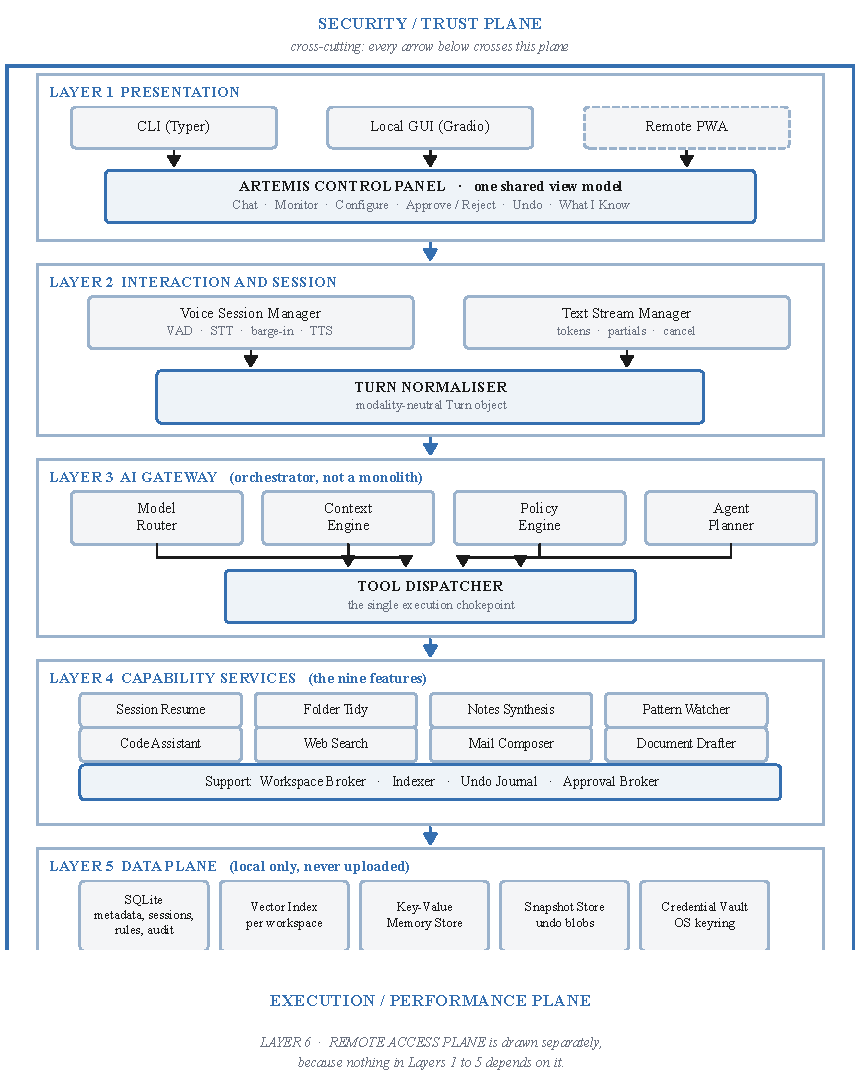
\includegraphics[width=0.72\textwidth]{Figures/fig_layers.pdf}
    \caption{The layered architecture. Layers one to five form the local execution path, the two planes cross every layer, and the remote access plane is drawn outside the stack because removing it leaves a fully functional system.}
    \label{fig:layers}
\end{figure}

Security and performance are represented as planes rather than layers, and this is a deliberate representational choice. A layer is a stage a request passes through, and drawing security as a layer would imply that a request could be past security, which is precisely the reasoning error that produces confused-deputy defects. They are drawn as planes to indicate that every arrow in the architecture crosses both.

\section{Design Considerations}
\subsection{Assumptions and Dependencies}
The design depends on the following, each of which would require reconsideration were it to change.

\begin{itemize}
    \item The operating system's canonicalisation routine resolves symbolic links correctly, since the confinement guarantee is built upon it. The design does not depend on any platform-specific behaviour beyond this
    \item The relational store enforces referential integrity when instructed to do so, since revocation is expressed as a cascading deletion. Because the engine disables this by default, it must be enabled explicitly on every connection
    \item A local model runtime is available, or the user has enabled cloud fallback for the workspaces concerned. The router treats providers as configuration, so a change of provider is not a change of design
    \item The user is a single individual with authority over the folders they grant. The design does not address shared or concurrent access by multiple users
    \item Documents within a workspace may be adversarial, since a file may have originated anywhere. The design therefore treats all retrieved content as data rather than as instruction
    \item Functionality is expected to change most in the capability layer, as features are added. The uniform tool contract exists so that such change does not propagate into the gateway
\end{itemize}

\subsection{General Constraints}
The following constraints shaped the design, and the impact of each is stated.

\begin{itemize}
    \item \textbf{Resource envelope.} The system must remain usable on a consumer laptop, which requires that expensive work be asynchronous and that every queue be bounded. The impact is the execution plane described in Section 6.4
    \item \textbf{Offline operation.} Core functionality must not require connectivity, which requires that a local model be the default tier and that networked capabilities degrade explicitly. The impact is the degradation contract in Table~\ref{tab:degradation}
    \item \textbf{Data residency.} User data must not reach a project-operated server, which places egress enforcement in the router, where workspace policy is known, rather than in the tool layer
    \item \textbf{No inbound port.} The remote plane must dial outward, which determines the topology in Section 6.4 and removes any requirement for firewall configuration or network address translation traversal
    \item \textbf{Credential handling.} Secrets must reside in the operating system keyring, which excludes them from the system's own storage tree and from any backup of it
    \item \textbf{Verification.} Each guarantee must be testable, which requires that each have exactly one enforcement point. This is the reason resolution occurs in one component and execution in another
    \item \textbf{Team and timeline.} Three members across two semesters requires that the optional components be separable, which is why the remote plane is architecturally detachable
\end{itemize}

\subsection{Goals and Guidelines}
Four principles dominate the design, and the reason for each is stated because none is self-evident.

\emph{A property must be structural rather than promised.} Where a guarantee can be expressed as the absence of a code path rather than as a check, it is so expressed. This is why destructive operations have no approval dialogue: a check can be defeated by a defect or an unanticipated path, whereas an absent capability cannot.

\emph{Each guarantee has exactly one enforcement point.} Resolution occurs in the broker and nowhere else; execution occurs in the dispatcher and nowhere else. The reason is verification: a guarantee with two enforcement points has two opportunities to drift apart, and no single place at which it can be audited.

\emph{Legibility is a component of trust.} Background work reports visible, cancellable progress, the disclosure panel is a live query rather than a written summary, and the audit log records refusals as well as actions. The reason is that a system whose behaviour cannot be observed cannot be trusted regardless of its actual correctness.

\emph{The failure mode is refusal.} An unrecognised operation is denied, an unresolvable path is refused, a full queue sheds work visibly, and an expired approval can never execute. The reason is that permissive failure in a system holding a boundary converts a defect into a breach.

\subsection{Development Methods}
The design was produced by deriving structure from the research findings and the specification rather than by adapting a reference architecture. The layered form with cross-cutting planes is conventional, and the component decomposition within the gateway follows from a specific requirement: the original design made a single component responsible for routing, context, memory, planning, policy and dispatch simultaneously, which was untestable because no individual guarantee could be isolated. The decomposition into four components with a single shared execution point was adopted to make each guarantee separately verifiable. This revision also introduced the policy engine as a first-class component, converting the approval-first finding from an interface behaviour into enforced structure.

\section{System Architecture}
The system's responsibilities are partitioned so that each guarantee is held by exactly one component. Table~\ref{tab:components} presents the component inventory, stating for each component its layer, its responsibility and the single thing it must never do. The final column is the operative one: it states the invariant whose violation would constitute a defect in the architecture rather than in the implementation.

\begin{table}[!ht]
\centering
\caption{Component inventory, stating the layer, responsibility and governing invariant of each component.}
\label{tab:components}
{\small
\begin{tabular}{|p{0.6cm}|p{2.8cm}|p{0.9cm}|p{4.0cm}|p{4.2cm}|}
\hline
\textbf{\#} & \textbf{Component} & \textbf{Layer} & \textbf{Responsibility} & \textbf{Must never} \\
\hline
1 & Command line interface & 1 & Scriptable control surface & Bypass the approval broker \\
\hline
2 & Graphical control panel & 1 & Visual control surface, loopback-bound & Bind to a non-loopback interface \\
\hline
3 & Control panel view model & 1 & Single source of interface truth across surfaces & Hold state the backend does not own \\
\hline
4 & Voice session manager & 2 & Activity detection, transcription, interruption, synthesis & Record when not explicitly armed \\
\hline
5 & Text stream manager & 2 & Token streaming and cancellation & Buffer past a cancellation \\
\hline
6 & Turn normaliser & 2 & Produce the modality-neutral turn & Leak modality downstream \\
\hline
7 & Model router & 3 & Select a tier and fail over; enforce egress & Send workspace data to a disabled tier \\
\hline
8 & Context engine & 3 & Assemble bounded, cited context & Include content outside the grant \\
\hline
9 & Policy engine & 3 & Classify risk and decide gating & Be consulted after execution \\
\hline
10 & Agent planner & 3 & Produce a multi-step plan & Execute anything itself \\
\hline
11 & Tool dispatcher & 3 & Sole execution point & Accept a call lacking a policy verdict \\
\hline
12 & Capability services & 4 & The features & Touch the filesystem directly \\
\hline
13 & Workspace broker & 4 & Path resolution and confinement & Resolve a path outside a grant \\
\hline
14 & Indexer & 4 & Incremental indexing and embedding & Block the interactive path \\
\hline
15 & Undo journal & 4 & Snapshots and inverse operations & Record an action after the fact \\
\hline
16 & Approval broker & 4 & Hold pending actions and fan out to surfaces & Approve on timeout \\
\hline
17 & Data plane stores & 5 & Local persistence & Serialise outside the host \\
\hline
18 & Remote access plane & 6 & Authenticated relay & Store or read plaintext user data \\
\hline
\end{tabular}}
\end{table}

The collaboration between these components is expressed by the request lifecycle shown in Figure~\ref{fig:lifecycle}, which is the single most important path in the system. Every request, whether spoken or typed and whether local or remote, traverses exactly this sequence, and no shortcut exists.

\begin{figure}[!ht]
    \centering
    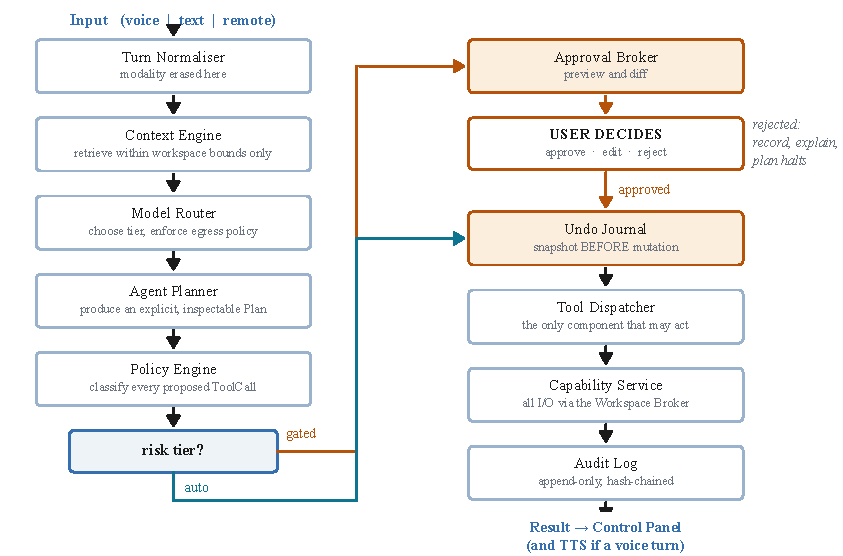
\includegraphics[width=0.86\textwidth]{Figures/fig_lifecycle.pdf}
    \caption{The request lifecycle. Modality is erased at the turn normaliser, the policy engine is consulted before the dispatcher, the snapshot precedes the mutation, and the audit entry is written whether the action proceeds or is refused.}
    \label{fig:lifecycle}
\end{figure}

Five invariants are enforced along this path, and together they constitute the architecture's guarantees. The policy engine is consulted before the dispatcher and never after. The undo journal records its snapshot before the mutation and never after. The audit entry is written even when the action is rejected, so the log records what was proposed rather than only what occurred. A call lacking a matching policy verdict is refused by the dispatcher. Voice and text turns are indistinguishable from the planner onward, which is what renders voice parity structural rather than a second implementation.

The decomposition was chosen over two alternatives. A single orchestrating component was rejected because no individual guarantee could be isolated for testing, and because a defect anywhere within it would compromise every guarantee simultaneously. A per-feature arrangement, in which each capability held its own gating logic, was rejected because it would produce as many enforcement points as features, none of which could be audited centrally, and each of which could drift.

\subsection{Subsystem Architecture: The Gateway}
The gateway is decomposed into four components with a single shared execution point, as shown in Figure~\ref{fig:gateway}. The planner produces a plan and cannot execute it; the dispatcher executes and cannot plan; the policy engine renders a verdict on each proposed call; and the router determines which model tier may be used and whether data may leave the machine.

\begin{figure}[!ht]
    \centering
    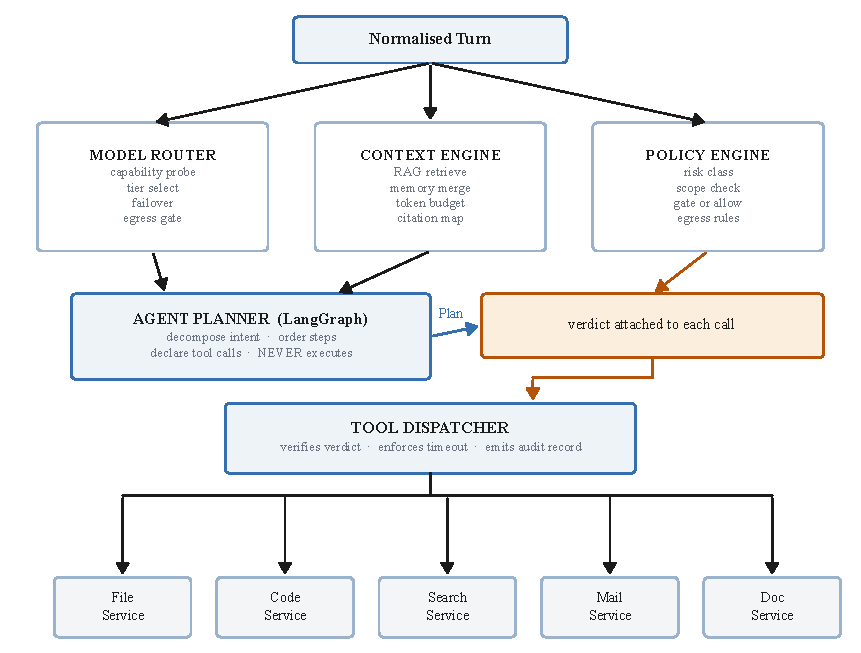
\includegraphics[width=0.68\textwidth]{Figures/fig_gateway.pdf}
    \caption{Internal structure of the gateway. The planner produces a plan but never executes it, and every call converges on the dispatcher, which is the sole execution point.}
    \label{fig:gateway}
\end{figure}

The model router owns tier selection and egress enforcement. Egress is enforced here, rather than in the tool layer or in the prompt, because the router is the component that knows a given workspace's cloud policy. Tier zero is the local model and is the default. Higher tiers are reachable only where the workspace permits, and any compatible endpoint may be registered as an additional tier without modification to the code, since providers are treated as configuration rather than as branches. Failover is bounded at one retry per tier before advancing, so a workspace with cloud disabled possesses exactly one tier and its failure produces a clean degradation message rather than an indefinite wait. Figure~\ref{fig:router} shows the selection and the egress gate.

\begin{figure}[!ht]
    \centering
    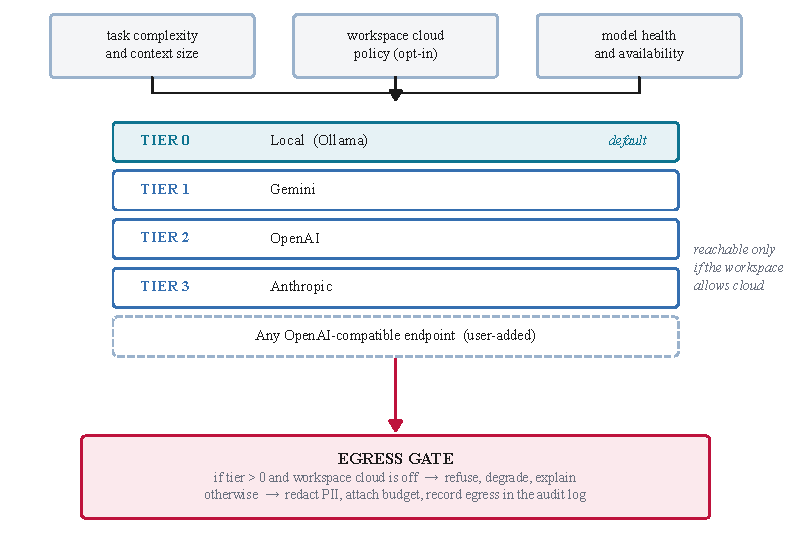
\includegraphics[width=\linewidth]{Figures/fig_router.pdf}
    \caption{Tier selection and the egress gate. Tiers above zero are reachable only where the workspace's cloud policy permits, and every egress is recorded.}
    \label{fig:router}
\end{figure}

The context engine assembles the model's working context and enforces bounded scope on the read side, as the broker does on the write side. Every retrieved chunk carries the identifier of the workspace it came from, and any chunk not matching the active grant is discarded and the discard recorded. A token budgeter weights by recency and relevance but never truncates a citation source silently. A citation map carries each chunk back to its file and line, and this map is what makes the synthesis feature verifiable, since a claim that cannot be traced through it is rendered as unsupported rather than presented as established. Figure~\ref{fig:context} shows this assembly.

\begin{figure}[!ht]
    \centering
    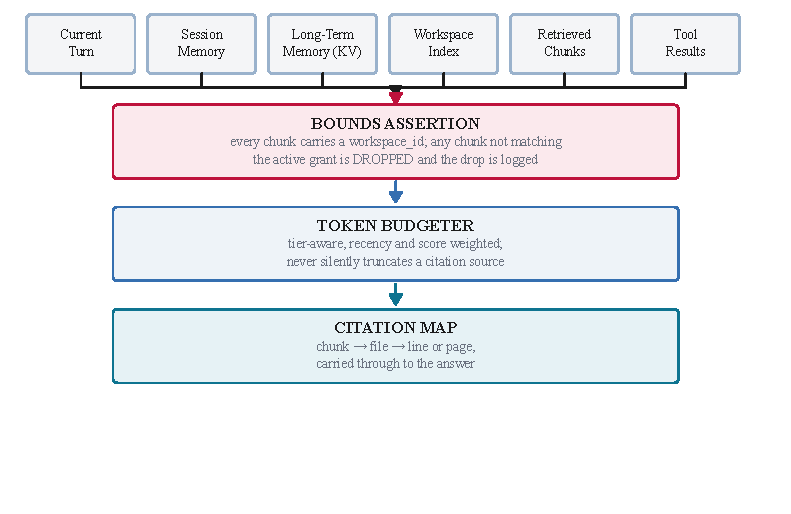
\includegraphics[width=\linewidth]{Figures/fig_context.pdf}
    \caption{Context assembly. Every retrieved chunk carries a workspace identifier, any chunk outside the active grant is discarded and the discard logged, and the citation map is carried through to the answer.}
    \label{fig:context}
\end{figure}

The policy engine classifies each proposed call according to the procedure stated in Chapter 5. Figure~\ref{fig:tiers} presents the four tiers and Figure~\ref{fig:policyorder} the evaluation order in which denials precede gates and gates precede permissions.

\begin{figure}[!ht]
    \centering
    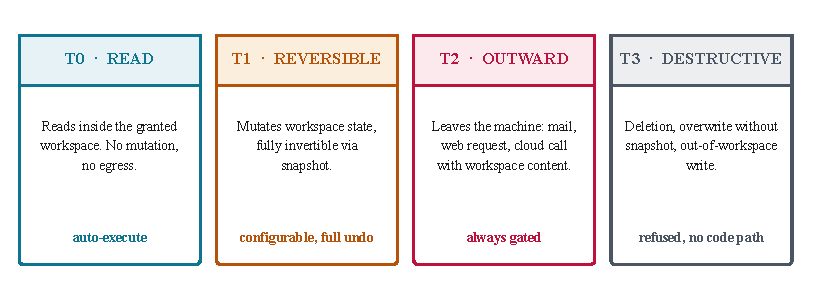
\includegraphics[width=\linewidth]{Figures/fig_tiers.pdf}
    \caption{The four risk tiers. Only the reversible tier is user-configurable; outward actions are always gated and destructive actions are structurally unavailable.}
    \label{fig:tiers}
\end{figure}

\begin{figure}[!ht]
    \centering
    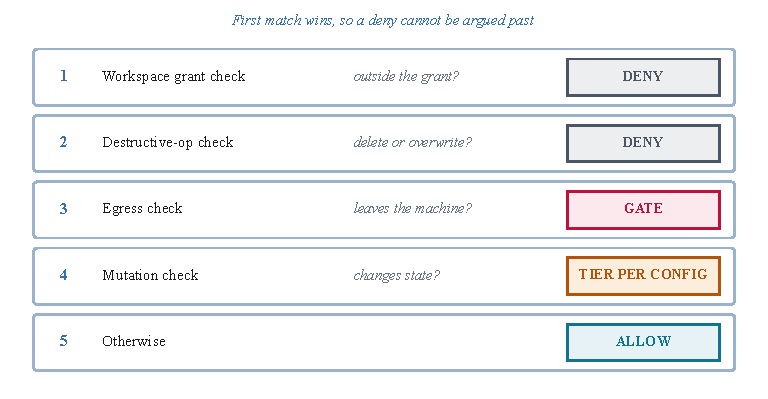
\includegraphics[width=\linewidth]{Figures/fig_policy_order.pdf}
    \caption{Policy evaluation order. Denials are evaluated before gates and gates before permissions, so that the first match is the decision and no later rule can grant what an earlier rule refused.}
    \label{fig:policyorder}
\end{figure}

Figure~\ref{fig:approval} shows a worked classification for a folder tidy, in which the read steps execute automatically and the two state-changing steps are gated, producing a preview that states what will occur and, equally importantly, what will not.

\begin{figure}[!ht]
    \centering
    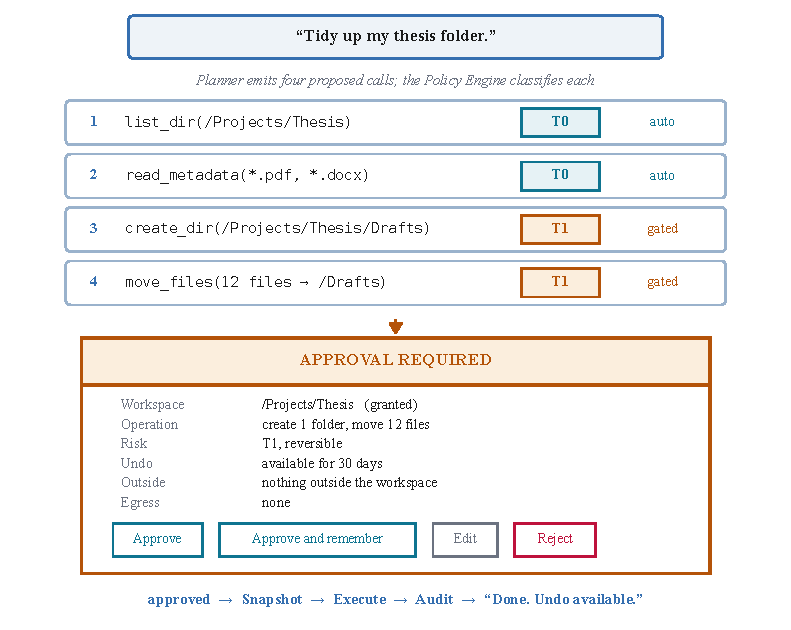
\includegraphics[width=0.62\textwidth]{Figures/fig_approval.pdf}
    \caption{A worked classification and approval for a folder tidy. Read operations execute automatically while the reversible operations are gated, and the preview states that nothing leaves the machine and nothing is deleted.}
    \label{fig:approval}
\end{figure}

The agent planner produces plans using LangGraph and never executes them. Its reflection loop is bounded by an explicit cycle cap and a wall-clock budget, which addresses the repetitive-loop failure mode the planning literature reports: an agent unable to converge surfaces its partial plan and asks, rather than looping indefinitely.

\subsection{Subsystem Architecture: Capability Services}
The features are implemented as services behind a uniform tool contract. None touches the filesystem, the network or the database directly; each reaches them through the shared substrate of the broker, the journal, the approval broker and the data plane, as shown in Figure~\ref{fig:services}.

\begin{figure}[!ht]
    \centering
    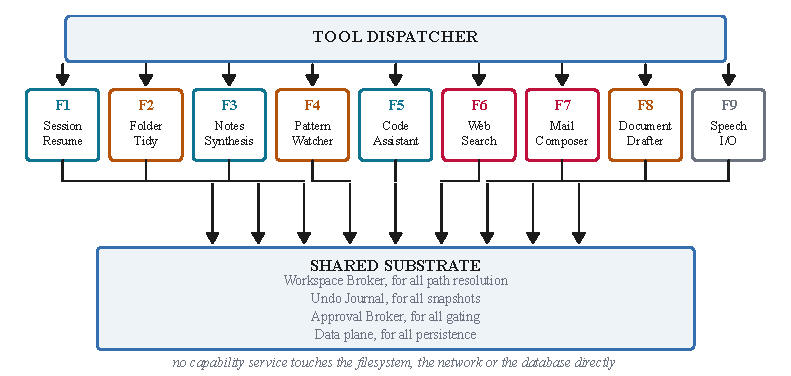
\includegraphics[width=\linewidth]{Figures/fig_services.pdf}
    \caption{Capability services are reachable only through the tool dispatcher and reach the filesystem only through the shared substrate, so no service holds its own path to the filesystem.}
    \label{fig:services}
\end{figure}

Table~\ref{tab:services} states the highest tier each service may request. The table is a design constraint rather than a description: a service cannot request a tier above its stated maximum, which is what confines the consequences of a defect within any one feature.

\begin{table}[!ht]
\centering
\caption{The capability services and the highest risk tier each may request.}
\label{tab:services}
\begin{tabular}{|p{0.9cm}|p{3.4cm}|p{1.6cm}|p{6.4cm}|}
\hline
\textbf{\#} & \textbf{Service} & \textbf{Max tier} & \textbf{Notes} \\
\hline
F1 & Session resume & T0 & Deterministic replay of recorded session state; no model involved \\
\hline
F2 & Folder tidy & T1 & Moves and groups only; no code path to deletion \\
\hline
F3 & Notes synthesis & T0 & Reads and generates; output remains a proposal until the drafter writes it \\
\hline
F4 & Pattern watcher & T1 & Detects three or more repetitions and may only propose a rule; cannot install one \\
\hline
F5 & Code assistant & T0 & Explains and produces a difference; never writes and never executes \\
\hline
F6 & Web search & T2 & On demand only; every query recorded \\
\hline
F7 & Mail composer & T2 & Draft, approve, send; sending is gated regardless of configuration \\
\hline
F8 & Document drafter & T1 & Always writes a new file; never overwrites an existing one \\
\hline
F9 & Speech input and output & Not applicable & Not a service but a modality at layer two, over identical gates \\
\hline
\end{tabular}
\end{table}

That the ninth feature is not a service is a deliberate structural claim. Voice is normalised at the interaction layer into the same turn object as text, so it inherits every approval gate automatically. Parity is thereby achieved by construction rather than by reimplementing the gates along a second path, and the stage seven gate described in Chapter 5 exists to test precisely this.

The workspace broker is the component that turns a logical reference into a real path, and Figure~\ref{fig:broker} shows its five assertions. The ordering of the second and third is the entire substance of the guarantee: canonicalising before testing containment is what resolves a symbolic link or a traversal segment to its true location before the test occurs.

\begin{figure}[!ht]
    \centering
    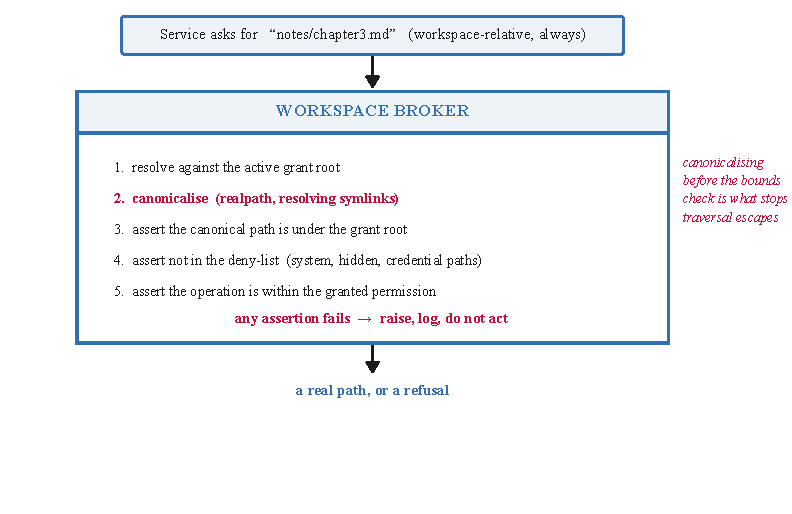
\includegraphics[width=\linewidth]{Figures/fig_broker.pdf}
    \caption{Path resolution and confinement. Canonicalisation occurs before the containment test, which is what distinguishes a boundary from a suggestion.}
    \label{fig:broker}
\end{figure}

\section{Architectural Strategies}
This section states the strategies that shaped the architecture, the reasoning behind each, and the alternatives considered and rejected.

\subsection{Local-First Operation with Optional Egress}
The system defaults to a local model and treats cloud access as a per-workspace opt-in. The reasoning is threefold: the research reported local-first as the most common deployment preference, privacy appeared as both a churn risk and a recurring free-text concern, and offline operation is a stated constraint.

The alternative of cloud-first operation with a local fallback was rejected because it inverts the guarantee. Under that arrangement the default behaviour transmits user data and the user must act to prevent it, whereas the chosen arrangement requires action to permit it. The trade-off accepted is capability: a small local model performs less well than a large hosted one, which is mitigated by bounded failover where the workspace permits and by honest degradation where it does not.

The degradation contract in Table~\ref{tab:degradation} states the required behaviour as each external capability is withdrawn. Each row is a testable acceptance criterion rather than an aspiration, and together they define the system's correctness under adverse conditions.

\begin{table}[!ht]
\centering
\caption{The degradation contract: required behaviour as each external capability is withdrawn.}
\label{tab:degradation}
{\small
\begin{tabular}{|p{4.6cm}|p{8.6cm}|}
\hline
\textbf{Withdrawn capability} & \textbf{Required behaviour} \\
\hline
Internet connectivity & Full local operation continues. Cloud model calls, web search and mail sending are disabled, each failing as an explicit retryable action rather than being silently dropped \\
\hline
All cloud model providers & Falls back to the local model. Features exceeding local capability degrade to a stated limitation rather than an error \\
\hline
Local model & Falls forward to the cloud chain, if and only if the workspace permits cloud access \\
\hline
Remote device & The host continues uninterrupted. Approvals in flight revert to pending and appear on the host surface \\
\hline
Remote edge & Local operation is entirely unaffected, because the remote plane is not on the execution path \\
\hline
Workspace grant & The system cannot see the folder. Not declines to touch it: the path is not resolvable at all \\
\hline
\end{tabular}}
\end{table}

\subsection{Separation of Memory from the File Index}
The system maintains two distinct kinds of knowledge, and conflating them is the error that converts a bounded assistant into a surveillance instrument. Figure~\ref{fig:memory} shows the five kinds of memory and Figure~\ref{fig:memoryindex} the distinction that matters.

\begin{figure}[!ht]
    \centering
    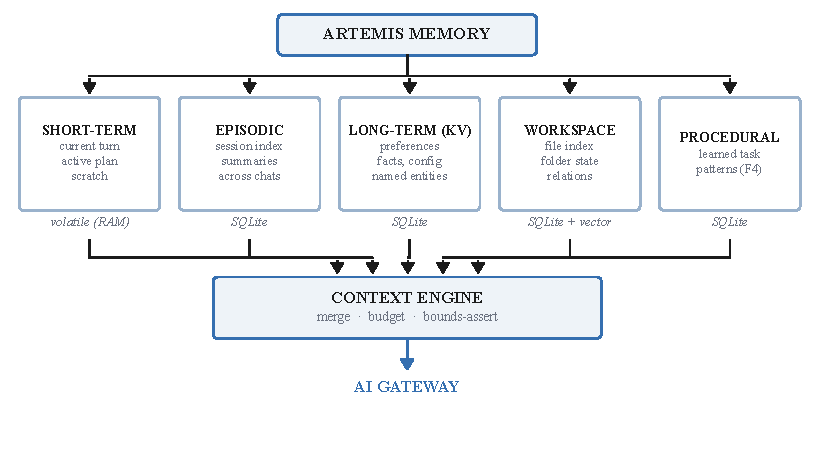
\includegraphics[width=\linewidth]{Figures/fig_memory.pdf}
    \caption{Five kinds of memory distinguished by lifetime and by store, all feeding a single context engine that merges, budgets and asserts bounds.}
    \label{fig:memory}
\end{figure}

\begin{figure}[!ht]
    \centering
    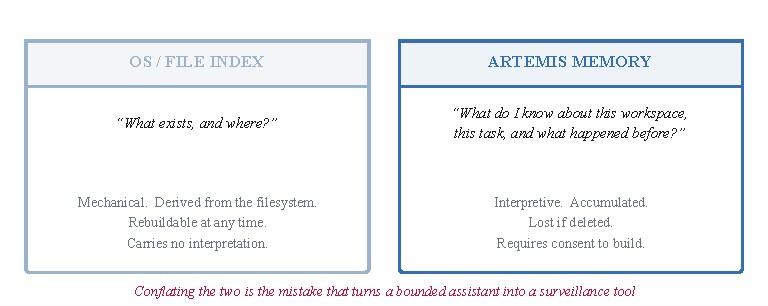
\includegraphics[width=\linewidth]{Figures/fig_memory_vs_index.pdf}
    \caption{The file index and system memory answer different questions and carry different consequences. The index is mechanical and rebuildable; memory is interpretive and, once deleted, lost.}
    \label{fig:memoryindex}
\end{figure}

The file index answers what exists and where. It is mechanical, derived from the filesystem, rebuildable at any time, and carries no interpretation. Memory answers what the system has learned about a workspace, a task and a user's preferences. It is interpretive, accumulated, lost if deleted, and requires consent to build. The design keeps them in separate stores with separate lifecycles, and every memory entry is individually visible and deletable in the disclosure panel. This is also how the most requested unmet capability, that the system learn the user's organisational habits, is accommodated without widening the boundary: such learning is per-workspace memory, subject to the same visibility and deletion as everything else.

\subsection{Disclosure as a Live Query}
The disclosure panel is not a summary the system writes about itself but a live query across every store. The reasoning is that a written summary can be stale or incorrect, whereas a query cannot disagree with the data it reads. Every row is deletable and deletion is a genuine cascade, so revoking a workspace removes its index directory, its file rows, its embeddings and its memory entries.

The alternative of a periodically generated report was rejected because it would make the trust claim persuasive rather than falsifiable, and a falsifiable claim is the stronger position. The audit log is deliberately excluded from deletion, on the principle that a log its subject can erase is not an audit log.

\subsection{The Remote Plane as a Detachable Component}
The remote access plane is drawn outside the core stack, and the test of whether that separation is genuine is that removing the entire plane leaves a fully functional single-machine system. Figure~\ref{fig:remote} shows its structure and Figure~\ref{fig:pairing} the pairing handshake.

\begin{figure}[!ht]
    \centering
    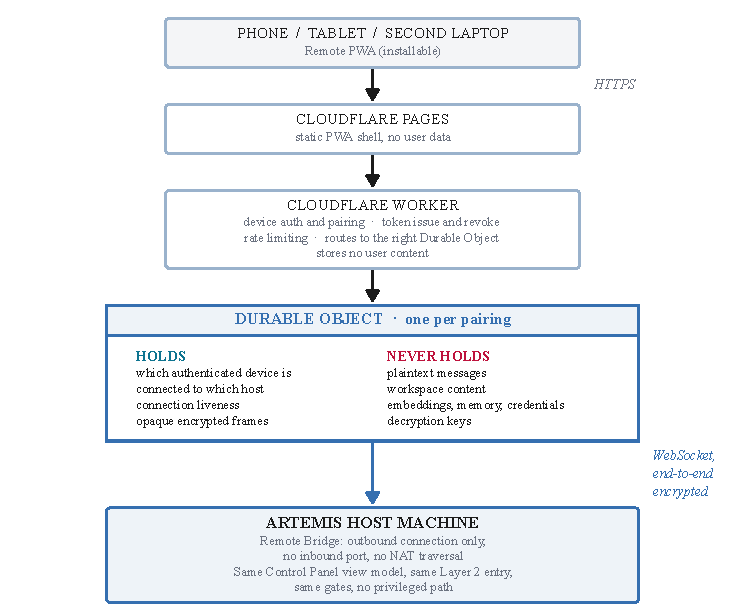
\includegraphics[width=0.48\textwidth]{Figures/fig_remote.pdf}
    \caption{The remote access plane. The durable object records which authenticated device is connected to which host and relays encrypted frames it cannot read.}
    \label{fig:remote}
\end{figure}

\begin{figure}[!ht]
    \centering
    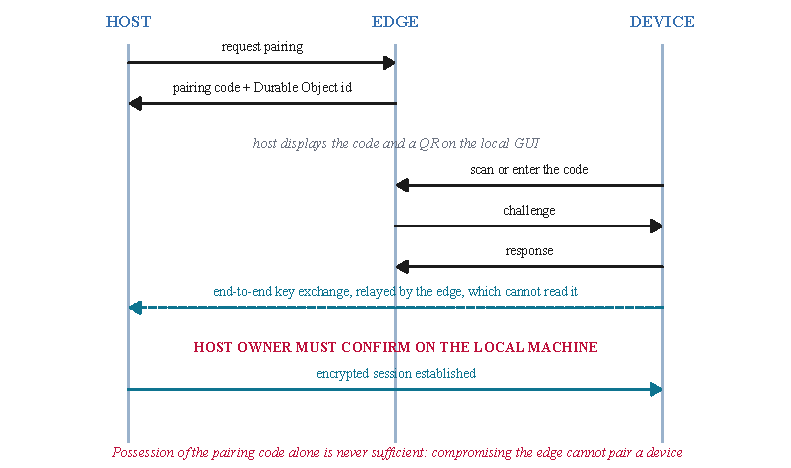
\includegraphics[width=\linewidth]{Figures/fig_pairing.pdf}
    \caption{The pairing handshake. Host-side confirmation is deliberate, so that possession of the pairing code alone is never sufficient to pair a device.}
    \label{fig:pairing}
\end{figure}

The plane is a control surface rather than a privilege escalation. Remote sessions run at equal or lower privilege than local ones and never higher. A workspace may be marked local-only, rendering it invisible to remote sessions. Outward actions may be configured to require local approval regardless of where they were requested, and this is the default. Sessions expire on a fixed interval and on host sleep, revocation is instant and unilateral from the host, and every remote-originated action is tagged with its device in the audit log. The relay holds no plaintext, so the privacy claim survives compromise of the edge.

\subsection{Asynchrony with Bounded Queues}
The interactive path remains thin and everything expensive is asynchronous, as shown in Figure~\ref{fig:performance}. Indexing is incremental, re-embedding only chunks whose content hash has changed, so a one-line edit re-embeds one chunk rather than a file. Retrieval is two-stage, with inexpensive vector recall followed by a reranking pass, which keeps the index small while maintaining quality. The local model is held resident with an idle timer so that the first token does not pay a cold load.

\begin{figure}[!ht]
    \centering
    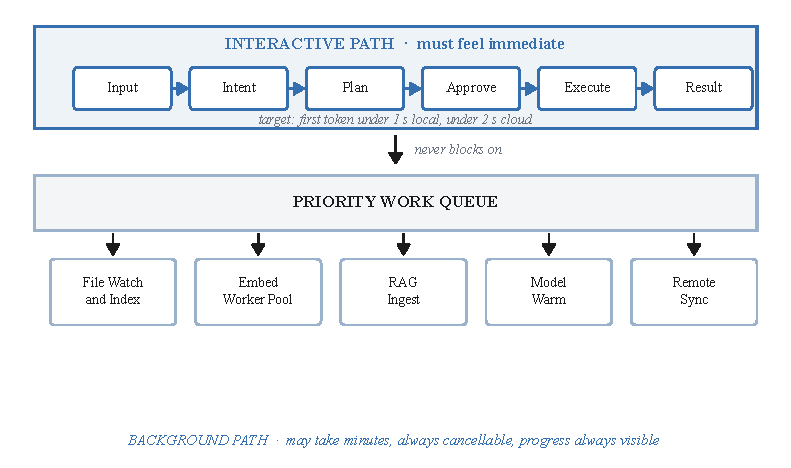
\includegraphics[width=0.66\textwidth]{Figures/fig_performance.pdf}
    \caption{The interactive path never blocks on background work, and background progress is reported visibly and remains cancellable.}
    \label{fig:performance}
\end{figure}

Every queue is bounded, and a full queue sheds its lowest-priority work and reports having done so rather than growing without limit. The reasoning is that unbounded queues convert a load problem into a memory exhaustion problem, and that a system which silently falls behind is one whose behaviour the user cannot predict.

\section{Domain Model/Class Diagram}
The domain model is centred on four immutable value objects and five services that operate upon them. The value objects are immutable by design, so that a verdict cannot be attached to one call and the call then altered before it runs.

A \emph{ToolCall} represents one proposed action, carrying an operation name, a workspace identifier, a set of paths relative to that workspace, arguments and a unique identifier. Its paths are relative rather than absolute, so that a call cannot smuggle an absolute path past the boundary by careful construction. It provides a description for previews and logs, and a fingerprint identifying the shape of the call independently of the paths it touches, which is the scope at which remembered approvals apply.

A \emph{Verdict} represents the policy engine's conclusion about one call, carrying the call identifier it was issued for, the tier, the decision, the reason and the rule applied. It exposes whether approval is required and whether the call was refused, and it can confirm that it corresponds to a given call. That correspondence check is what prevents a call being classified as a read and then executed as something else.

A \emph{Plan} is an ordered collection of calls with an intent and an identifier, and it is the unit at which approval and reversal operate.

A \emph{Resolved} path is one that has passed every assertion of the broker. Services accept this type rather than a bare path, so that an unchecked path cannot reach the filesystem by accident. Holding one is the proof that the boundary was tested.

The services are the \emph{WorkspaceBroker}, which resolves references or refuses; the \emph{PolicyEngine}, which classifies calls and holds remembered rules; the \emph{ApprovalBroker}, which holds pending plans, constructs previews and records decisions; the \emph{UndoJournal}, which records inverse operations and replays them; and the \emph{ToolDispatcher}, which is the only component that acts.

Two relationships in this model carry the architecture's guarantees. The dispatcher depends upon the approval broker rather than accepting an approval flag from its caller, so that a service cannot assert its own permission. The dispatcher also resolves paths through the broker a second time, despite the policy engine having already done so, because the dispatcher must not depend upon an earlier component having performed its function correctly; that assumption is the substance of confused-deputy defects.

\section{Policies and Tactics}
This section states the policies and tactics that govern implementation. They do not alter the overall structure but determine the details of interface and implementation.

\subsection{Refusal as the Default Failure Mode}
Every ambiguous condition resolves to refusal. An unrecognised operation is denied rather than treated as a read. An unresolvable path is refused rather than attempted. A call whose verdict is missing or mismatched is refused. An expired approval can never execute, which is why expiry is a distinct outcome rather than a variety of rejection or a silent discard.

The alternative, permissive defaults with explicit denial lists, was rejected because a denial list must anticipate every dangerous operation whereas a permission list need only enumerate the safe ones, and the consequence of an omission differs in kind between the two.

\subsection{Single Enforcement Points}
Path resolution occurs in the broker alone and execution in the dispatcher alone. Handler registration is an allowlist, so an operation without a registered handler cannot run and adding a capability is a deliberate act rather than a consequence of a planner inventing a name.

This policy has a maintenance implication that must be stated for any future developer: introducing a second path to the filesystem or a second execution point would not be a refactoring but a change to what the system guarantees, and either would invalidate the testing strategy, which depends upon each guarantee having one place at which it can be verified.

\subsection{Ordering Constraints}
Three orderings are load-bearing and must not be altered. Canonicalisation precedes the containment test. The snapshot precedes the mutation. Policy evaluation precedes dispatch. Each of these is a correctness property rather than a stylistic preference, and reversing any of them produces a system that appears to function while providing none of the guarantee it claims. Each is therefore covered by a dedicated test whose purpose is to fail if the ordering is disturbed.

\subsection{Testing Strategy}
Testing is organised around the guarantees rather than around the code structure. The boundary is tested adversarially, with attempts to escape by relative traversal, by symbolic links pointing outside the grant, by absolute paths, and by sibling directories sharing a name prefix, each of which must be refused and recorded. Policy classification is tested exhaustively across the operation sets, including the unrecognised case. Approval is tested for the properties that nothing is approved by default and that outward operations cannot be remembered. Recovery is tested by executing a plan, reversing it, and comparing the result against the state recorded beforehand.

Each stage of the build sequence concludes with a gate test, and a stage is complete when its gate passes rather than when its code exists. Gates are formulated so that they are capable of failing, the clearest instance being the speech stage gate, which fails if voice required any new approval gate.

\subsection{Concurrency Handling}
The interactive path is single-threaded but the store is reached from more than one thread, because the file watcher flushes its debounce buffer on a timer. The store therefore serialises every statement behind a lock, and all access passes through its guarded methods rather than reaching the connection directly. Disabling the database engine's own thread guard without providing this lock would exchange a visible error for silent corruption, so the two belong together.

The audit log's chain read and append occur under a single lock, so that two threads cannot chain onto the same predecessor and fork the chain.

\subsection{Source Organisation}
The source is organised by architectural role rather than by feature, so that the correspondence between the design and the code is direct. Core components, being the broker, the policy engine, the approval broker, the undo journal, the dispatcher and the disclosure panel, reside in one package. The data plane resides in another. Interface surfaces reside in a third. A reader looking for the enforcement point of a guarantee finds it where the architecture says it is.


{
\bibliographystyle{ieeetr}
\bibliography{fypbib}
}

\appendix
\chapter{Research Instruments and Response Distributions}
This appendix records the instruments used in the foundational research and the complete response distributions summarised in Chapters 2 and 3. It is included so that the findings cited throughout the report can be examined at the level of the underlying data.

\section{Research Method}
The foundational research comprised two instruments. A questionnaire of seventeen items drew 374 valid responses, covering the respondent's context, the problem, design and trust preferences, and feature demand, with attitudinal items using a five-point scale. An interview guide coded thirteen in-person conversations on five axes: the last occasion on which the participant lost their place in multi-file work, the workaround they already employ, their reaction to the concept, the effect a trust-breaking mistake would have, and whether they would continue using the system.

Recruitment was through the institution's student and practitioner networks, and the questionnaire ran from 22 to 27 August 2026. Four limitations apply and are stated because they bound every conclusion drawn from this data. The sample is self-selected and drawn from a single institution. Students predominate, so the professional signal rests on a smaller subsample. The system was described in text rather than demonstrated, so predicted use and predicted churn are stated intentions rather than observed behaviour. Some free-text responses contain near-identical phrasings, which suggests that certain answers were presented as suggested text, so theme counts should be read as indicative.

\section{Respondent Profile}
Table~\ref{tab:appprofile} gives the composition of the sample and the frequency with which respondents perform multi-file work.

\begin{table}[!ht]
\centering
\caption{Respondent role and frequency of multi-file project work, from 374 valid responses.}
\label{tab:appprofile}
\begin{tabular}{|p{6.0cm}|r|r|}
\hline
\textbf{Response} & \textbf{Count} & \textbf{Percent} \\
\hline
\multicolumn{3}{|l|}{\textbf{Role}} \\
\hline
Student & 302 & 80.7 \\
\hline
Developer or software engineer & 47 & 12.6 \\
\hline
Freelance & 12 & 3.2 \\
\hline
Employed & 7 & 1.9 \\
\hline
Other & 6 & 1.6 \\
\hline
\multicolumn{3}{|l|}{\textbf{Frequency of multi-file project work}} \\
\hline
Daily & 147 & 39.3 \\
\hline
A few times a week & 159 & 42.5 \\
\hline
A few times a month & 68 & 18.2 \\
\hline
\multicolumn{3}{|l|}{\textbf{Prior use of an AI assistant}} \\
\hline
Yes, regularly & 172 & 46.0 \\
\hline
Yes, occasionally & 115 & 30.7 \\
\hline
Tried once or twice & 48 & 12.8 \\
\hline
Never & 39 & 10.4 \\
\hline
\end{tabular}
\end{table}

\section{Headline Findings}
The nine findings established by the research, referenced throughout Chapters 2 and 4, are as follows.

\begin{itemize}
    \item \textbf{F1.} The reorientation problem is real. 44 percent of respondents struggle to recall what they were doing on returning to a project after a break, and only 7 percent never do
    \item \textbf{F2.} File disorder outpaces manual cleanup for 59 percent of respondents
    \item \textbf{F3.} The problem costs real time at moderate scale, with 42 percent losing more than an hour a week and 14 percent more than three hours
    \item \textbf{F4.} The work is unautomated because of distrust of automation at 36 percent and lack of know-how at 28 percent, rather than because the tasks do not exist
    \item \textbf{F5.} The bounded-workspace hypothesis holds. 65 percent rate a workspace-only assistant more trustworthy than a full-access one, with a mean of 3.8, and 40 percent prefer local-first operation
    \item \textbf{F6.} Users are forgiving of a single mistake. 65 percent would continue using the system after one wrong suggestion and only 10 percent would abandon it
    \item \textbf{F7.} The principal retention risks are habit fit at 27 percent and an untrusted mistake at 24 percent; approval fatigue is real but smaller at 10 percent
    \item \textbf{F8.} Feature demand is concentrated on session resume, notes synthesis and folder tidy, with speech last by a wide margin
    \item \textbf{F9.} The interviews confirm the questionnaire and add effortless onboarding as a named condition for continued use
\end{itemize}

\section{Segment Analysis}
Table~\ref{tab:appsegments} presents selected measures by respondent segment. Role does not predict the interaction preference, since students and developers give near-identical workspace-trust ratings and identical approval-first shares. Experience moves it modestly: regular users of assistants prefer approval-first less often than light or non-users, which is consistent with heavier users being more comfortable delegating. The effect is small and neither group approaches unanimity, so the practical conclusion is unchanged, which is that the interaction model must be a setting rather than a fixed decision.

\begin{table}[!ht]
\centering
\caption{Selected measures by respondent segment.}
\label{tab:appsegments}
\begin{tabular}{|p{5.2cm}|r|p{2.4cm}|p{2.2cm}|p{2.0cm}|}
\hline
\textbf{Segment} & \textbf{n} & \textbf{Workspace trust (mean)} & \textbf{Prefer approval-first} & \textbf{Prefer local-first} \\
\hline
All respondents & 374 & 3.8 & 51\% & 40\% \\
\hline
Students & 302 & 3.8 & 51\% & 41\% \\
\hline
Developers and engineers & 47 & 3.7 & 51\% & 36\% \\
\hline
Regular assistant users & 172 & 3.9 & 44\% & 40\% \\
\hline
Light or non-users & 87 & 3.8 & 59\% & 41\% \\
\hline
\end{tabular}
\end{table}

\section{Interview Findings}
Figure~\ref{fig:interview} presents the coded interview responses. Ten of the thirteen participants reacted positively to the concept, with the remainder split between conditional, mixed and one negative response. Eight of thirteen said a single mistake would not stop them, several qualifying this with caution, while two said a trust-breaking mistake would cause them to stop. Six said outright that they would continue using the system and four said they would do so conditionally, with effortless onboarding named as the most common condition, followed by privacy and by the system reaching sufficient maturity.

\begin{figure}[!ht]
    \centering
    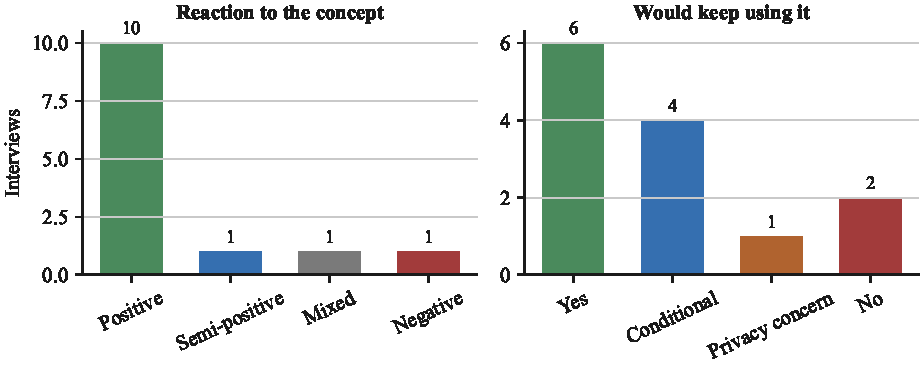
\includegraphics[width=\textwidth]{Figures/fig_interview.pdf}
    \caption{Coded interview responses across thirteen interviews, showing reaction to the concept and whether the participant would continue using the system.}
    \label{fig:interview}
\end{figure}

The workarounds participants already employ were consistent: informal notes written by hand or with an assistant to record where they left off, repeated manual restructuring because every project has a different structure, and simply tolerating the friction because automating it appears to cost more than it saves.

\section{Additional Response Distributions}
Figures~\ref{fig:messy}, \ref{fig:wstrust}, \ref{fig:localcloud}, \ref{fig:mistake}, \ref{fig:likely}, \ref{fig:churn} and \ref{fig:themes} present the remaining distributions underlying the findings cited in Chapters 2 and 4.

\begin{figure}[!ht]
    \centering
    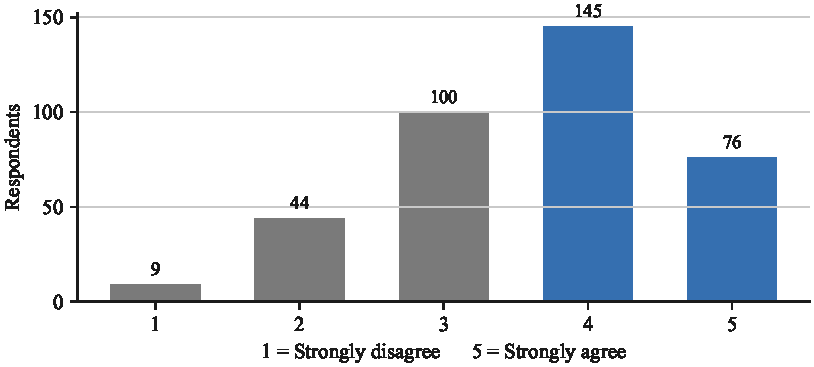
\includegraphics[width=0.82\textwidth]{Figures/fig_messy_agree.pdf}
    \caption{Agreement that folders and files become disorganised faster than they can be manually cleaned, on a five-point scale.}
    \label{fig:messy}
\end{figure}

\begin{figure}[!ht]
    \centering
    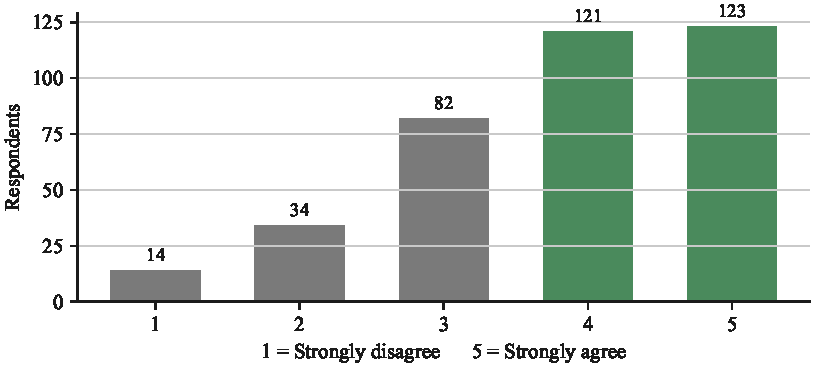
\includegraphics[width=0.82\textwidth]{Figures/fig_workspace_trust.pdf}
    \caption{Agreement that an assistant seeing only explicitly added files is meaningfully more trustworthy than one with full machine access. This is the most direct test of the project's central hypothesis.}
    \label{fig:wstrust}
\end{figure}

\begin{figure}[!ht]
    \centering
    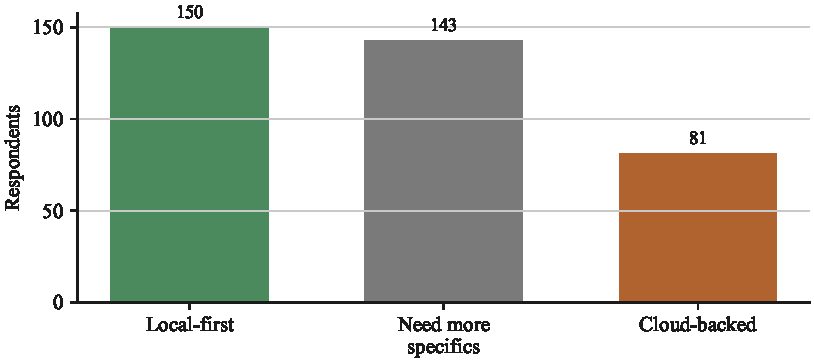
\includegraphics[width=0.82\textwidth]{Figures/fig_local_vs_cloud.pdf}
    \caption{Preference between a local, offline-first version and a cloud-backed version.}
    \label{fig:localcloud}
\end{figure}

\begin{figure}[!ht]
    \centering
    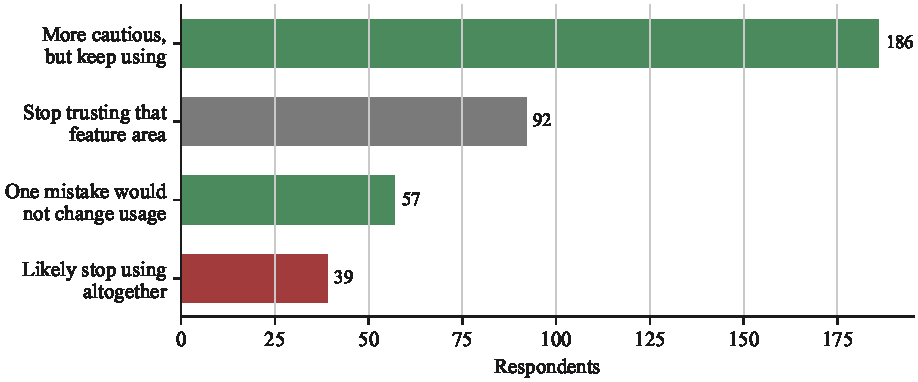
\includegraphics[width=\textwidth]{Figures/fig_wrong_suggestion.pdf}
    \caption{Reported response to a single wrong or unwanted suggestion, such as incorrectly grouped files or a mistake in a drafted message.}
    \label{fig:mistake}
\end{figure}

\begin{figure}[!ht]
    \centering
    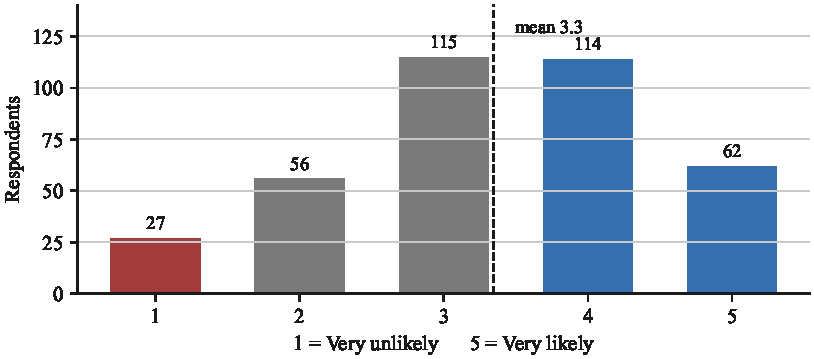
\includegraphics[width=0.82\textwidth]{Figures/fig_likely_use.pdf}
    \caption{Likelihood of continued use after the novelty has passed, assuming the system worked as described, on a five-point scale.}
    \label{fig:likely}
\end{figure}

\begin{figure}[!ht]
    \centering
    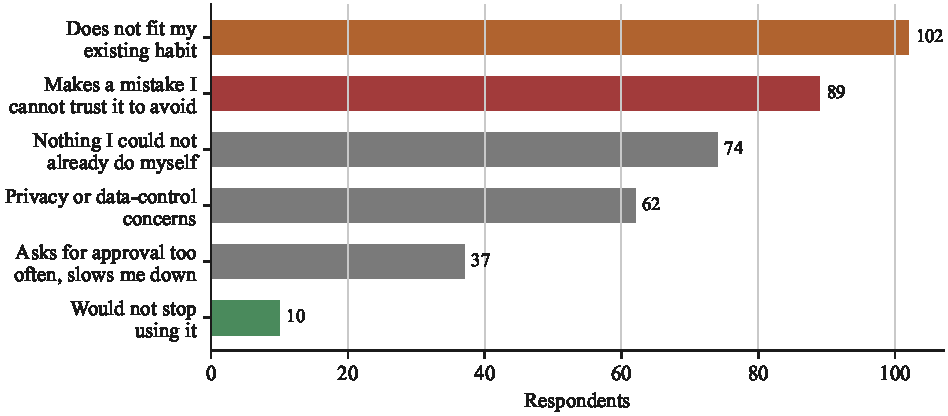
\includegraphics[width=\textwidth]{Figures/fig_stop_reason.pdf}
    \caption{The single most likely reason a respondent would stop using the system after a week.}
    \label{fig:churn}
\end{figure}

\begin{figure}[!ht]
    \centering
    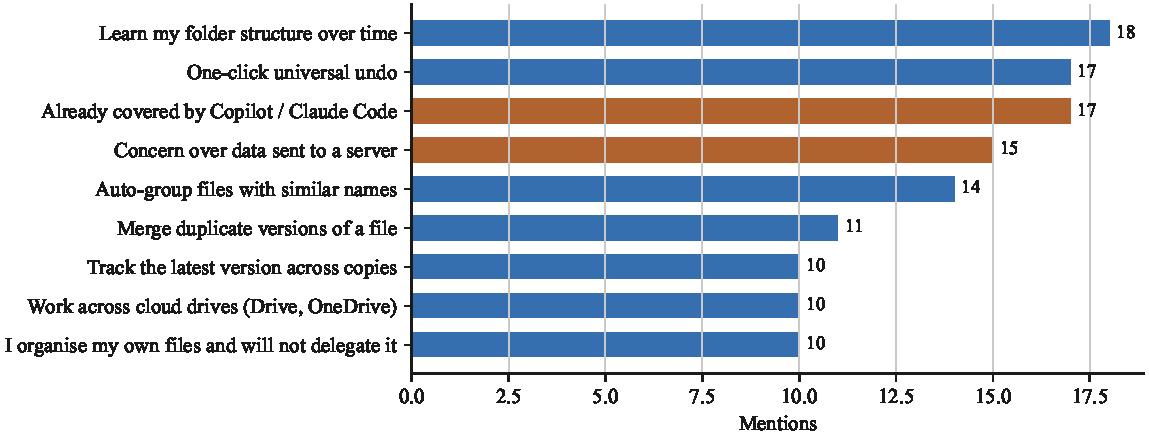
\includegraphics[width=\textwidth]{Figures/fig_open_feedback_themes.pdf}
    \caption{Recurring themes in free-text responses. Counts are indicative given repeated phrasings in the raw data.}
    \label{fig:themes}
\end{figure}

\end{document}
